\documentclass[final]{cpecmu}
%% This is a sample document demonstrating how to use the CPECMU
%% project template. If you are having trouble, see "cpecmu.pdf" for
%% documentation.

\projectNo{P808-2}
\acadyear{2023}

\titleTH{รับฟังฉันที ได้โปรด: เกมสยองขวัญมุมมองบุคคลที่ 3 แบบด้านข้าง}
\titleEN{Attention please: 3D side scrolling horror game}

\author{นายปริญญา ม่วงรอด}{Parinya Muangrod}{630612104}
\author{นางสาววิภาวี วรรธนัจฉริยา}{Wipawee Wattanutchariya}{630612190}

\cpeadvisor{karn}
\cpecommittee{navadon}
\cpecommittee{sakgasit}
%% Some possible packages to include:
\usepackage[final]{graphicx} % for including graphics

%% Add bookmarks and hyperlinks in the document.
\PassOptionsToPackage{hyphens}{url}
\usepackage[colorlinks=true,allcolors=Blue4,citecolor=red,linktoc=all]{hyperref}
\def\UrlLeft#1\UrlRight{$#1$}

%% Needed just by this example, but maybe not by most reports
\usepackage{afterpage} % for outputting
\usepackage{pdflscape} % for landscape figures and tables. 

%% Some other useful packages. Look these up to find out how to use
%% them.
% \usepackage{natbib}    % for author-year citation styles
% \usepackage{txfonts}
% \usepackage{appendix}  % for appendices on a per-chapter basis
% \usepackage{xtab}      % for tables that go over multiple pages
% \usepackage{subfigure} % for subfigures within a figure
% \usepackage{pstricks,pdftricks} % for access to special PostScript and PDF commands
% \usepackage{nomencl}   % if you have a list of abbreviations

%% if you're having problems with overfull boxes, you may need to increase
%% the tolerance to 9999
% \tolerance=9999

% \bibliographystyle{plain}
% \bibliographystyle{IEEEbib}
\bibliographystyle{IEEEtran}

% \renewcommand{\topfraction}{0.85}
% \renewcommand{\textfraction}{0.1}
% \renewcommand{\floatpagefraction}{0.75}

%% Example for glossary entry
%% Need to use glossary option
%% See glossaries package for complete documentation.
\ifglossary
  \newglossaryentry{lorem ipsum}{
    name=lorem ipsum,
    description={derived from Latin dolorem ipsum, translated as ``pain itself''}
  }
\fi

%% Uncomment this command to preview only specified LaTeX file(s)
%% imported with \include command below.
%% Any other file imported via \include but not specified here will not
%% be previewed.
%% Useful if your report is large, as you might not want to build
%% the entire file when editing a certain part of your report.
% \includeonly{chapters/intro,chapters/background}

\begin{document}
\maketitle
\makesignature

\ifproject
    \begin{abstractTH}
        % เขียนบทคัดย่อของโครงงานที่นี่

        เกมแนวสยองขวัญ เป็นเกมที่จะมีเรื่องราวให้ผู้เล่นได้สวมบทบาทและเผชิญหน้ากับสิ่งที่น่าหวาดกลัว ความกดดัน และเอาตัวรอดจากสถานการณ์ต่าง ๆ ในเกม 
        ซึ่งเป็นแนวเกมที่ได้รับความนิยมในยุคปัจจุบัน โดยในโครงงานนี้ จะเป็นการพัฒนาเกมแนวสยองขวัญ ที่มีมุมมองบุคคลที่ 3 แบบด้านข้าง โดยผู้เล่นจะได้รับบทบาทเป็นนักเรียนคนหนึ่ง 
        ที่มีเพื่อนสนิทพยายามฆ่าตัวตาย แต่ไม่สำเร็จ และนอนไม่ได้สติอยู่ในโรงพยาบาล ผู้เล่นจะต้องค้นหาความจริง โดยการไขปริศนาต่าง ๆ และต้องเอาตัวรอดจากอุปสรรคที่คอยรบกวนผู้เล่น 
        ไม่ให้ไปถึงความจริง และต้องการจะปลิดชีพผู้เล่น ระบบของเกมจะถูกออกแบบให้ผู้เล่นจะต้องคอยบริหารค่าพลังงานที่ใช้ในการทำกิจกรรมต่างๆ ค่าสติที่มีผลกับการรับรู้ของตัวละคร 
        และเวลาที่มีอยู่อย่างจำกัด ซึ่งข้อจำกัดเหล่านี้จะส่งผลให้ผู้เล่นมีความกดดันในการตัดสินใจเลือกการกระทำ สำหรับการดำเนินเนื้อเรื่องและฉากจบ จะมีการเปลี่ยนแปลงไปตามการเลือก ข้อมูล 
        และไอเทมที่ได้รับในระหว่างเล่นเกม โดยเกมนี้ถูกพัฒนาขึ้นด้วยโปรแกรม Unity และภาษา C$\#$ เกมถูกออกแบบมาสำหรับผู้ที่มีอายุ 18 ปีขึ้นไป และเล่นบน PC โดยผู้พัฒนาคาดหวังว่า 
        ผู้เล่นจะได้รับความบันเทิง ความสนุก และข้อคิดจากเรื่องราวที่ปรากฏภายในเกม
        % การเขียนรายงานเป็นส่วนหนึ่งของการทำโครงงานวิศวกรรมคอมพิวเตอร์
        % เพื่อทบทวนทฤษฎีที่เกี่ยวข้อง อธิบายขั้นตอนวิธีแก้ปัญหาเชิงวิศวกรรม และวิเคราะห์และสรุปผลการทดลองอุปกรณ์และระบบต่างๆ
        % \enskip อย่างไรก็ดี การสร้างรูปเล่มรายงานให้ถูกรูปแบบนั้นเป็นขั้นตอนที่ยุ่งยาก
        % แม้ว่าจะมีต้นแบบสำหรับใช้ในโปรแกรม Microsoft Word แล้วก็ตาม
        % แต่นักศึกษาส่วนใหญ่ยังคงค้นพบว่าการใช้งานมีความซับซ้อน และเกิดความผิดพลาดในการจัดรูปแบบ กำหนดเลขหัวข้อ และสร้างสารบัญอยู่
        % \enskip ภาควิชาวิศวกรรมคอมพิวเตอร์จึงได้จัดทำต้นแบบรูปเล่มรายงานโดยใช้ระบบจัดเตรียมเอกสาร
        % \LaTeX{} เพื่อช่วยให้นักศึกษาเขียนรายงานได้อย่างสะดวกและรวดเร็วมากยิ่งขึ้น
    \end{abstractTH}

    \begin{abstract}
        A horror-themed game is a game where players take on roles and confront terrifying situations, pressure, and strive various scenarios in the game.
        This genre pf games has gained popularity in recent time. In this project, the development will focus on creating a third-person horror game perspective.
        Plyers will take on the role of a student who, after surviving an attempted suicide by their close friend, losesconsciousness and wake up in a hospital.
        Plyers will have to uncover the truth by solving various mysteries and obstacles that hider thier path to the truth.
        They must also navigate through challenges that attempt to thwart thier progress and endanger thier lives, as someone seeks to eliminate them.
        The game system is designed so that players must manage their energy levels of various activities, their character's awareness, and the limited available time. 
        These constraints lead players to experience pressure when making decisions. 
        The progression of the storyline and the ending scenes will change based on the choices made, information, and items obtained during gameplay will also influence these outcomes.
        This game is developed using the Unity and C$\#$ language.
        The game is designed for players aged 18 and above. And it is playable on PC.
        The developers aim to provide enterment, fun, and throught-provoking experiences through the storyline presented within the game.

        long (not counting the heading), and must not take up more than one (1) page
        (even if fewer than 350 words long).

        Make sure your abstract sits inside the \texttt{abstract} environment.
    \end{abstract}

    \iffalse
        \begin{dedication}
            This document is dedicated to all Chiang Mai University students.

            Dedication page is optional.
        \end{dedication}
    \fi % \iffalse

    \begin{acknowledgments}
        Your acknowledgments go here. Make sure it sits inside the
        \texttt{acknowledgment} environment.

        \acksign{2020}{5}{25}
    \end{acknowledgments}%
\fi % \ifproject

\contentspage

\ifproject
    \figurelistpage

    \tablelistpage
\fi % \ifproject

% \abbrlist % this page is optional

% \symlist % this page is optional

% \preface % this section is optional


\pagestyle{empty}\cleardoublepage
\normalspacing \setcounter{page}{1} \pagenumbering{arabic} \pagestyle{cpecmu}

\chapter{\ifenglish Introduction\else บทนำ\fi}

\section{\ifenglish Project rationale\else ที่มาของโครงงาน\fi}

\section{\ifenglish Objectives\else วัตถุประสงค์ของโครงงาน\fi}
\begin{enumerate}
    \item
\end{enumerate}

\section{\ifenglish Project scope\else ขอบเขตของโครงงาน\fi}

\subsection{\ifenglish Hardware scope\else ขอบเขตด้านฮาร์ดแวร์\fi}

\subsection{\ifenglish Software scope\else ขอบเขตด้านซอฟต์แวร์\fi}

\section{\ifenglish Expected outcomes\else ประโยชน์ที่ได้รับ\fi}

\section{\ifenglish Technology and tools\else เทคโนโลยีและเครื่องมือที่ใช้\fi}

\subsection{\ifenglish Hardware technology\else เทคโนโลยีด้านฮาร์ดแวร์\fi}

\subsection{\ifenglish Software technology\else เทคโนโลยีด้านซอฟต์แวร์\fi}

\section{\ifenglish Project plan\else แผนการดำเนินงาน\fi}

\begin{plan}{6}{2020}{2}{2021}
    \planitem{7}{2020}{8}{2020}{ศึกษาค้นคว้า}
    \planitem{8}{2020}{1}{2021}{ชิล}
    \planitem{2}{2021}{2}{2021}{เผา}
    \planitem{12}{2019}{1}{2022}{ทดสอบ}
\end{plan}

\section{\ifenglish Roles and responsibilities\else บทบาทและความรับผิดชอบ\fi}
อธิบายว่าในการทำงาน นศ. มีการกำหนดบทบาทและแบ่งหน้าที่งานอย่างไรในการทำงาน จำเป็นต้องใช้ความรู้ใดในการทำงานบ้าง

\section{\ifenglish%
Impacts of this project on society, health, safety, legal, and cultural issues
\else%
ผลกระทบด้านสังคม สุขภาพ ความปลอดภัย กฎหมาย และวัฒนธรรม
\fi}

แนวทางและโยชน์ในการประยุกต์ใช้งานโครงงานกับงานในด้านอื่นๆ รวมถึงผลกระทบในด้านสังคมและสิ่งแวดล้อมจากการใช้ความรู้ทางวิศวกรรมที่ได้

\chapter{\ifenglish Background Knowledge and Theory\else ทฤษฎีที่เกี่ยวข้อง\fi}

% การทำโครงงาน เริ่มต้นด้วยการศึกษาค้นคว้า ทฤษฎีที่เกี่ยวข้อง หรือ งานวิจัย/โครงงาน ที่เคยมีผู้นำเสนอไว้แล้ว ซึ่งเนื้อหาในบทนี้ก็จะเกี่ยวกับการอธิบายถึงสิ่งที่เกี่ยวข้องกับโครงงาน เพื่อให้ผู้อ่านเข้าใจเนื้อหาในบทถัดๆ ไปได้ง่ายขึ้น

\section{ทฤษฎีที่เกี่ยวข้อง}
\subsection{องค์ประกอบเกมสยองขวัญ} \cite{component-horror:theory} องค์ประกอบที่สำคัญมี ดังนี้
\begin{enumerate}
  \item เสียงและเพลงประกอบ เป็นส่วนประกอบหลักๆ ของการสร้างความสยองขวัญให้กับผู้เล่น ยกตัวอย่างเช่น เสียงพระสวดหรือดนตรีไทย ในเกม Home Sweet Home เป็นต้น
  \item ตัวละครที่ไร้ทางสู้ เป็นการเพิ่มความกดดันให้กับผู้เล่น เช่น สาวตาบอดหนีฆาตกรโรคจิตในเกม perception
  \item สถานที่ปิดตาย อาทิ ยานอาวกาศหรือจะเป็นโลกที่ถูกสร้างขึ้นมาอย่างบิดเบี้ยว สร้างความอึดอัด ไร้ทางหนี
  \item เรื่องราวที่มาที่ไปของความหายนะ ทุกๆเรื่องของความสยองขวัญ ต้องมีที่มาที่ไป เพื่อช่วยให้ผู้เล่นรู้สึกสยองขวัญ
  \item การแก้ไขปริศนา เกมแนวสยองขวัญเกือบจะทุกเกมนั้นต้องมีการแก้ไขปริศนาเพื่อหากุญแจที่จะนำมาเปิดประตู หรือหาสิ่งของมาเพื่อนำไปกระทำอะไรบางอย่าง เพื่อที่จะทำให้เราสามารถไปต่อได้
  \item เหยื่อผู้ร่วมชะตากรรม การเพิ่มตัวละครผู้เคราะห์ร้าย ที่อาจจะรอดหรือไม่รอดทำใ้หเราลุ้นจนจบ
  \item สิ่งของ อุปกรณ์ในการเอาตัวรอด ช่วยให้เราเอาตัวรอด บางอย่างก็เป็นอุปกรณ์ที่ใช้เเจ้งเตือนถึงบางสิ่งที่ไม่ประสงค์ดี
  \item เป้าหมาย เงื่อนไขที่เราต้องอยู่ที่แห่งนั้น เกมจำเป็นต้องมีเป้าหมาย เพื่อเป็นตัวกำหนดของการกระทำต่อๆไปของผู้เล่น
  \item อยู่ถูกที่ถูกเวลาหรือตรงตามเงื่อนไขที่ตัวร้ายกำหนด ตัวละครที่เราเป็นผู้เล่น เข้าไปติดกับดัก แล้วพบกับฆาตกรแบบพอดิบพอดี
\end{enumerate}

\section{เกมที่เกี่ยวข้อง}
\subsection{The Coma 2: Vicious sisters}
\subsubitem \textbf{The Coma 2:Vicious sisters} \cite{the-coma-2:theory} เป็นเกมแนว Survival Horror โดยผู้เล่นจะรับบทเป็นนักเรียนสาว พักมินอา ที่ตื่นขึ้นมาในโรงเรียนตอนดึก เธอได้รับรู้ถถึงสิ่งที่ผิดปกติ เธอพบว่ามีใครบางคนกำลังทำบางอย่าง ที่หน้าตาเหมือนอาจารย์ของเธอ พุ่งเข้ามาทำร้าย เธอจึงต้องหลบหนีเพื่อไม่ให้ถูกจับตัว โดยหนีไปในที่ที่ห่างออกไป แล้วพบกับสิ่งที่ทำให้ประหลาดใจมากมาย รวมไปถึงผู้ร่วมทางที่ดูไม่ค่อยเป็นมิตร จุดดเด่นของเกมนี้คือจะให้ผู้เล่นคอยหลบหนี จากการถูกจับตัว และจะมีสิ่งของให้ใช้เพื่อการอยู่รอด
\begin{figure}[h]
  \centering
  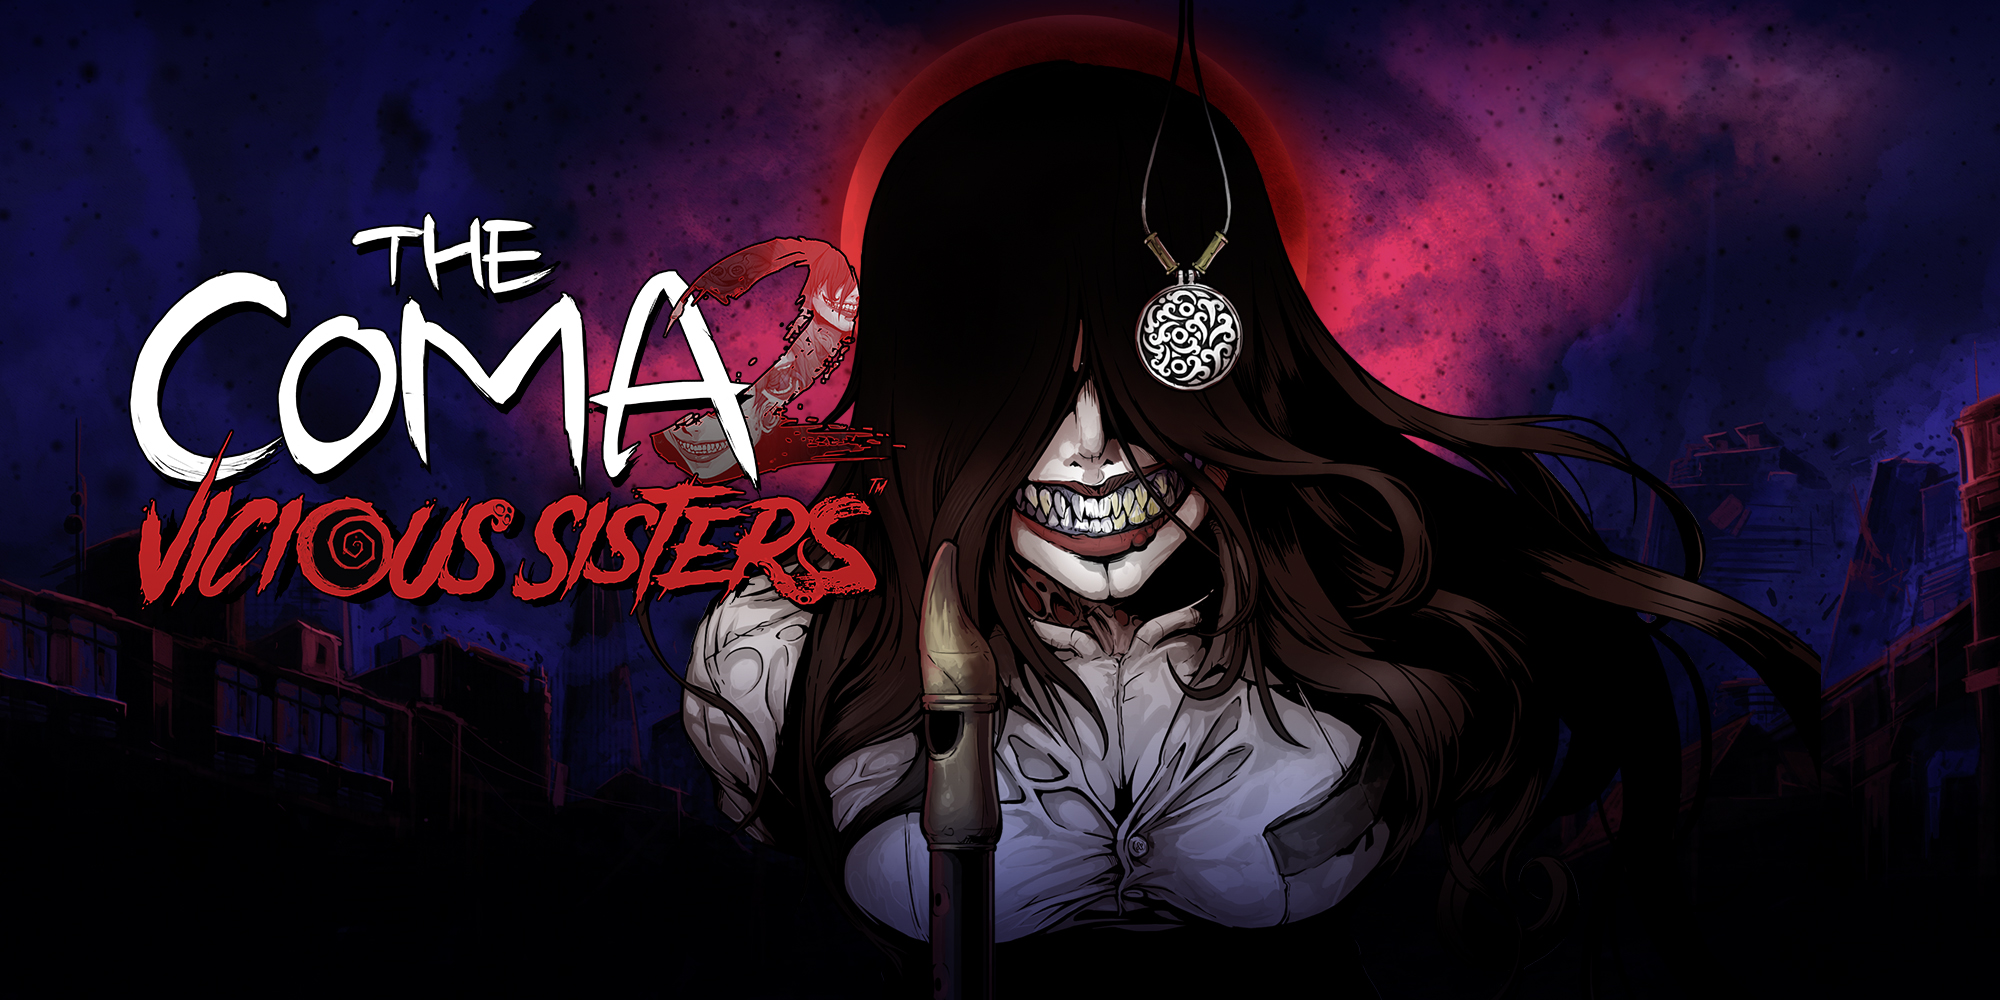
\includegraphics[width=0.6\textwidth, height=0.2\textheight]{Images/H2x1_NSwitchDS_TheComa2ViciousSisters.jpg}
  \caption{The Coma 2: Vicious sister จากเว็บไซต์}\label{TheComa2ViciousSisters}
\end{figure}

\subsection{Home Sweet Home}
\subsubitem \textbf{Home Sweet Home} \cite{home-sweet-home:theory} เป็นเกมแนว First Person, Adventure-Puzzle Horror โดยผู้เล่นจะรับบทเป็น ติม ที่ตื่นขึ้นมาในหอพักที่ไม่รู้จักมาก่อน เขาจึงออกสำรวจ แล้วได้เจอกับนักศึกษาสาว ที่อยู่ดีๆก็เข้ามาทำร้าย ทำให้ติมต้องหลบหนีออกจากหอพักแห่งนี้ ในระหว่างทางเขาได้พบกับเบาะแสบางอย่างที่ยังเป็นปริศณา หลังจากที่เขาได้หลบหนีออกมาได้ ติมก็ได้รู้สึกตัวอยู่ที่บ้านของเขา และได้รับสายฝากข้อความจากภรรยาของเขา เจน เจนได้หายตัวไป และได้ฝากไดอารี่ทิ้งไว้ ทำให้ติมต้องออกไปตามหาเจน ที่ระหว่างทางก็ได้พบกับเรื่องราวแปลกๆมากมาย ปริศณาว่าเจนอยู่ที่ไหน จุดเด่นของเกมจะเน้นไปที่การเล่าเรื่องราว และการหลบหนี/ซ่อนตัว จากภูติผีต่างๆที่จะมาออกล่า
\begin{figure}[h]
  \centering
  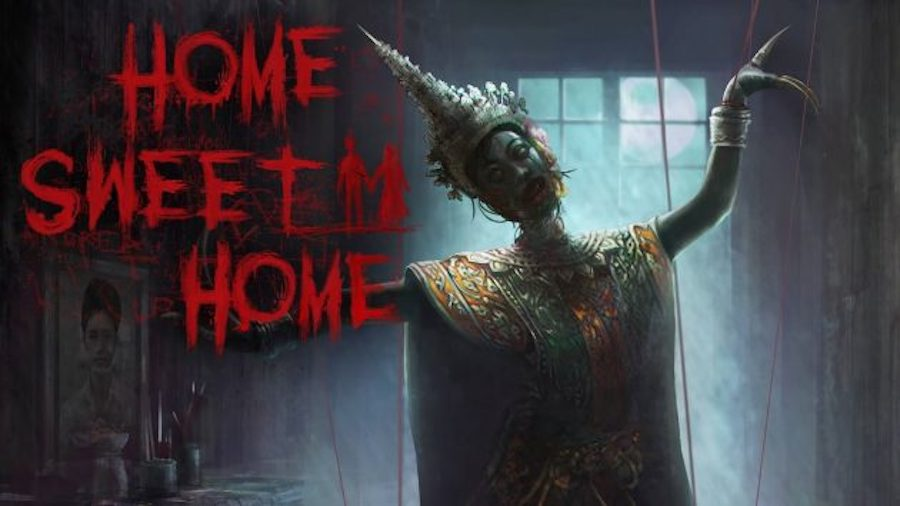
\includegraphics[width=0.6\textwidth, height=0.2\textheight]{Images/800px-HomeSweetHomePoster1.jpg}
  \caption{Home Sweet Home จากเว็บไซต์}\label{HomeSweetHomePoster1}
\end{figure}

\subsection{Outlast}
\subsubitem \textbf{Outlast} \cite{outlast:theory} เป็นเกมแนว First Person, Survival Horror โดยผู้เล่นจะรับบทเป็น Miles Upshur นักข่าวอิสระที่ได้รับข้อมูลจากแหล่งที่ไม่เปิดเผยตัวตน เขาจึงได้ลักลอบเข้าไปยัง Mount Massive Asylum บ้านร้างสำหรับคนป่าวโรคจิต และเขาก็ได้พบกับสิ่งที่น่าสะพรึงกลัวทั้งการทดลองที่ผิดจริยธรรมกับมนุษย์ ศาสนาที่บิดเบี่ยว วิญญาณผู้ป่วยทางจิต เขาจึงต้องหาทางออกไปจากสถานที่แห่งนี้ และนำเรื่องราวออกสู่โลกภายนอก จุดเเด่นของเกมนี้ ผู้เล่นจะต้องหาสิ่งของต่างๆ เพื่อนำมาปลดล็อคเส้นทางที่จะนำไปสู่การหลุดพ้น ผู้เล่นจะได้ใช้กล้องเพื่อบันทึกสิ่งต่างๆเพื่อเก็บข้อมูลที่จะคอยเฉลยเรื่องราวไปทีละส่วนๆ ผู้เล่นจะต้องคอยหลบซ่อนจากผู้ป่วยทางจิตและวิญญาณ
\begin{figure}[h]
  \centering
  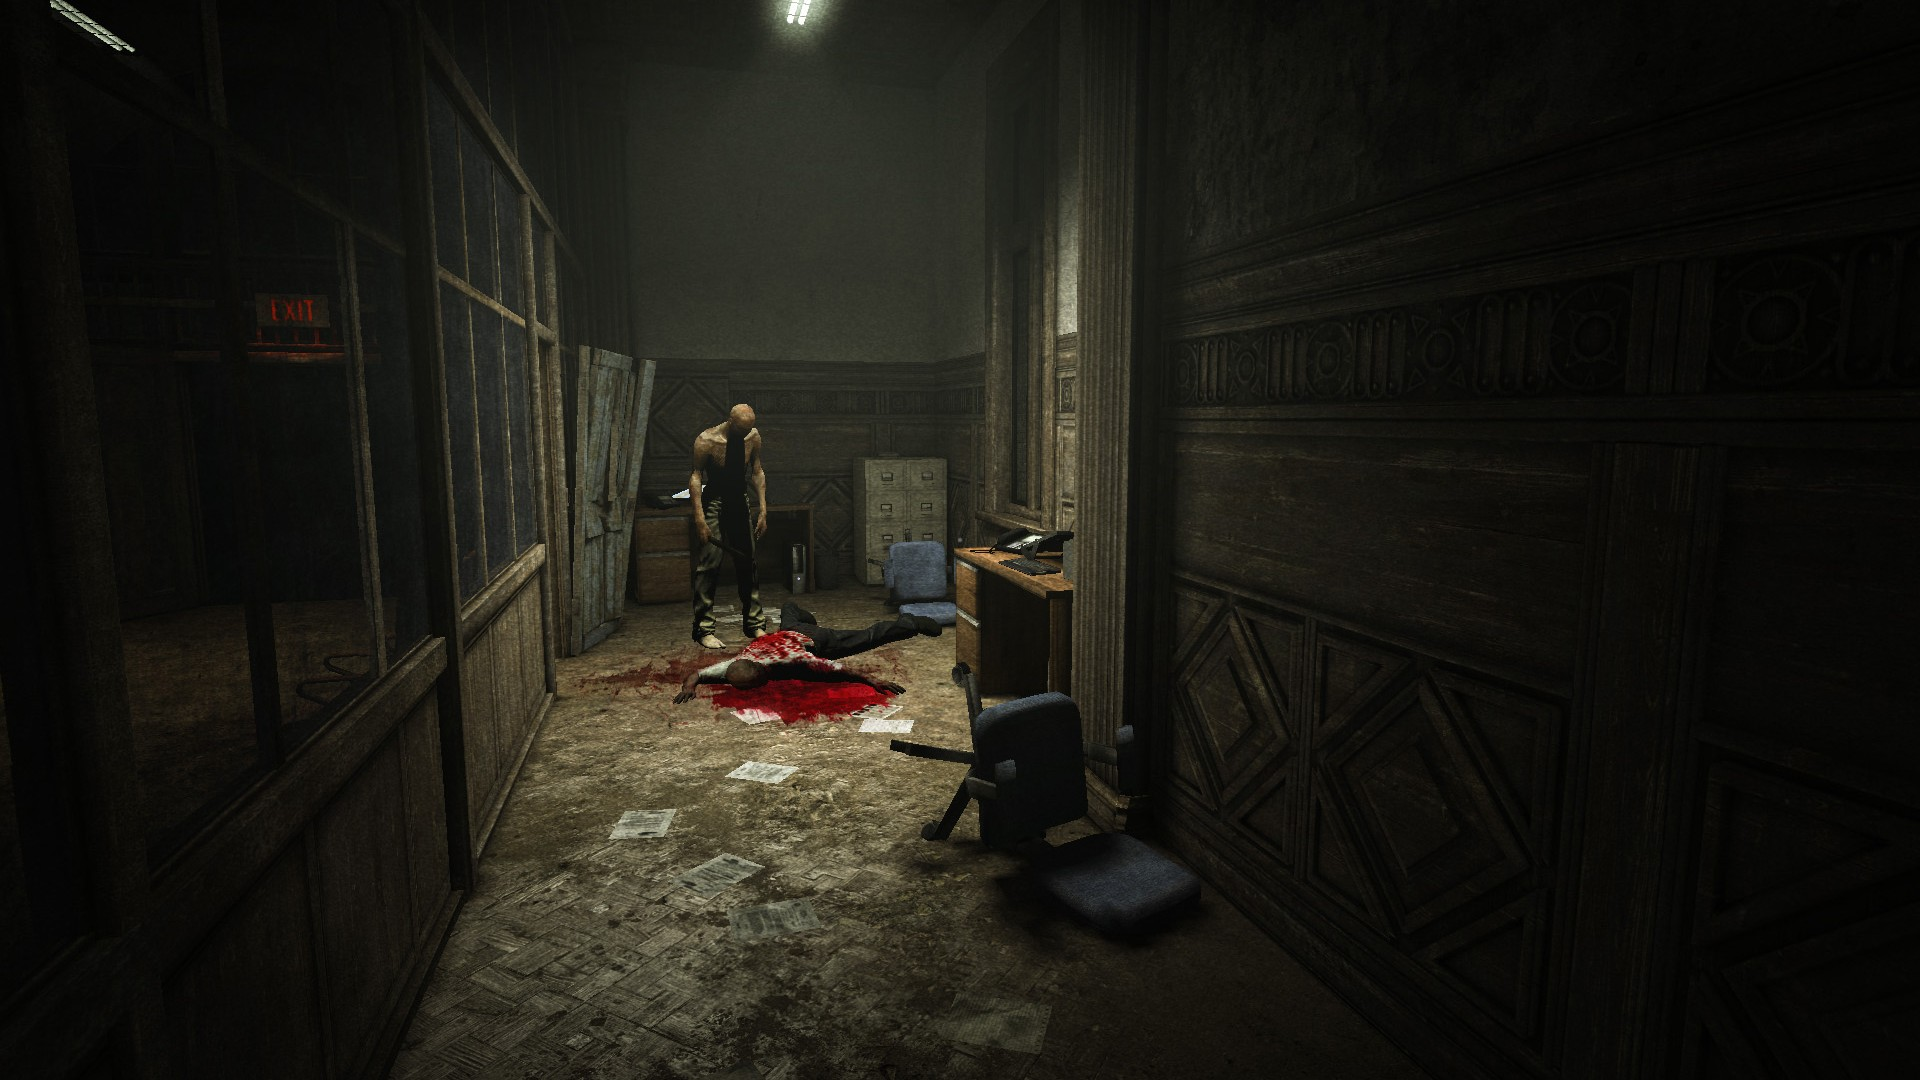
\includegraphics[width=0.6\textwidth, height=0.2\textheight]{Images/OutlastScreenShot-04-1920x1080.jpg}
  \caption{Outlast จากเว็บไซต์}\label{OutlastScreenShot}
\end{figure}

\subsection{Little Misfortune}
\subsubitem \textbf{Little Misfortune} \cite{outlast:theory} เป็นเกมประเภท side scrolling ซึ่งผู้เล่นจะได้รับบทเป็นหนูน้อย Little Misfortune ที่เป็นเด็กหญิงที่มีความมองโลกในแง่ดี เป็นคนสดใสร่าเริง ชอบแจกความสดใสโดยการโปรยกากเพชรใส่สิ่งของต่าง ๆ หนูน้อยจะออกเดินทางไปในเมืองซึ่งจะมีผู้ที่พูดคุยด้วย นั่นก็คือ Mr.Voice เขาจะนำทางหนูน้อยไปในที่ต่าง ๆ ซึ่งแรกๆก็ดูเหมือนจะเป็นเกมผจญภัยที่มีภาพน่ารักเหมือนการ์ตูนสำหรับเด็ก แต่เนื้อเรื่องกลับแฝงไปด้วยเนื้อหาของความบิดเบี้ยวของมนุษย์ ซึ่งประวัติของหนูน้อย Little Misfortune ก็คือเป็นเด็กที่เกิดมาโดยการท้องไม่พร้อม อีกทั้งยังมีความรุนแรงทางเพศและการใช้ภาษา การใช้ยาเสพติด เช่น บุหรี่ ซึ่งเป็นภาพที่หนูน้อยเห็นทุกวันจากแม่ที่ติดบุหรี่ และ Mr.Voice ที่หวังจะกลืนกินวิญญาณของหนูน้อยคนนี้ จึงหลอกเธอว่าเป็นเพื่อนที่ดี แต่ในโชคร้ายก็ยังมีโชคดีก็คือมีหมาจิ้งจอกตัวหนึ่งที่คอยช่วยเหลือหนูน้อยจาก Mr.Voice และในตอนจบของเรื่องก็ได้มีการเฉลยว่า อันที่จริงแล้ว หนูน้อย Little Misfortune ได้เสียชีวิตตั้งแต่เดินออกจากประตูบ้านไปแล้ว และคำว่า Little Misfortune ที่เธอใช้เรียกแทนตัวเอง ก็เป็นเพราะว่าตั้งแต่เธอเกิดมา ก็สร้างแต่ปัญหาและความทุกข์ให้ผู้เป็นแม่เนื่องจากการท้องไม่พร้อม แต่ถึงอย่างไรก็ตาม หนูน้อยคนนี้ก็ยังรักแม่ของเธอสุดหัวใจ และหวังว่าการตายของเธอจะทำให้แม่ของเธอมีความสุขมากขึ้น
\begin{figure}[h]
  \centering
  
\includegraphics[width=0.6\textwidth, height=0.2\textheight]{Images/little_misfortune.jpg}
  \caption{Little Misfortune จากเว็บไซต์}\label{little_misfurtune}
\end{figure}

\subsection{Martha is dead}
\subsubitem \textbf{Martha is dead} \cite{home-sweet-home:theory} เป็นเกมแนว First Person, Psychological Horror เกมนี้จะอยู่ในช่วงเวลาหลังสงครามโลกครั้งที่ 2 โดยผู้เล่นจะได้รับบทเป็น Giulia เนื้อเรื่องจะปูมาว่า Giulia มีฝาแฝดที่ชื่อว่า Martha ซึ่ง Martha เป็นลูกที่พ่อแม่รักมาก ๆ ต่างกับ Giulia ที่มีแต่ความเกลียดชัง อยู่มาวันหนึ่ง Martha ได้เสียชีวิตลงที่กลางทะเลสาย หลังจากนั้น Giulia ก็ต้องสืบหาความจริงว่าเกิดอะไรขึ้นกับ Martha โดยการปลอมตัวเป็น Martha และเธอก็ได้พบกับเรื่องราวต่าง ๆ มากมาย และภายหลังเกมก็จะค่อย ๆ เฉลยว่า จริงๆแล้ว Giulia ไม่ใช่ฝาแฝด แต่เป็นอีกบุคลิกที่ Martha สร้างขึ้นมาเพื่อหลบหนีจากความรุนแรงที่แม่ของเธอเคยทำร้ายเธอตอนเด็ก ๆ ซึ่งส่งผลให้ Martha นั้นมีบุคลิกที่คล้ายกับคนเป็นใบ้ หูหนวก ซึ่งต่างจาก Giulia ที่เป็นคนปกติ
\begin{figure}[h]
  \centering
  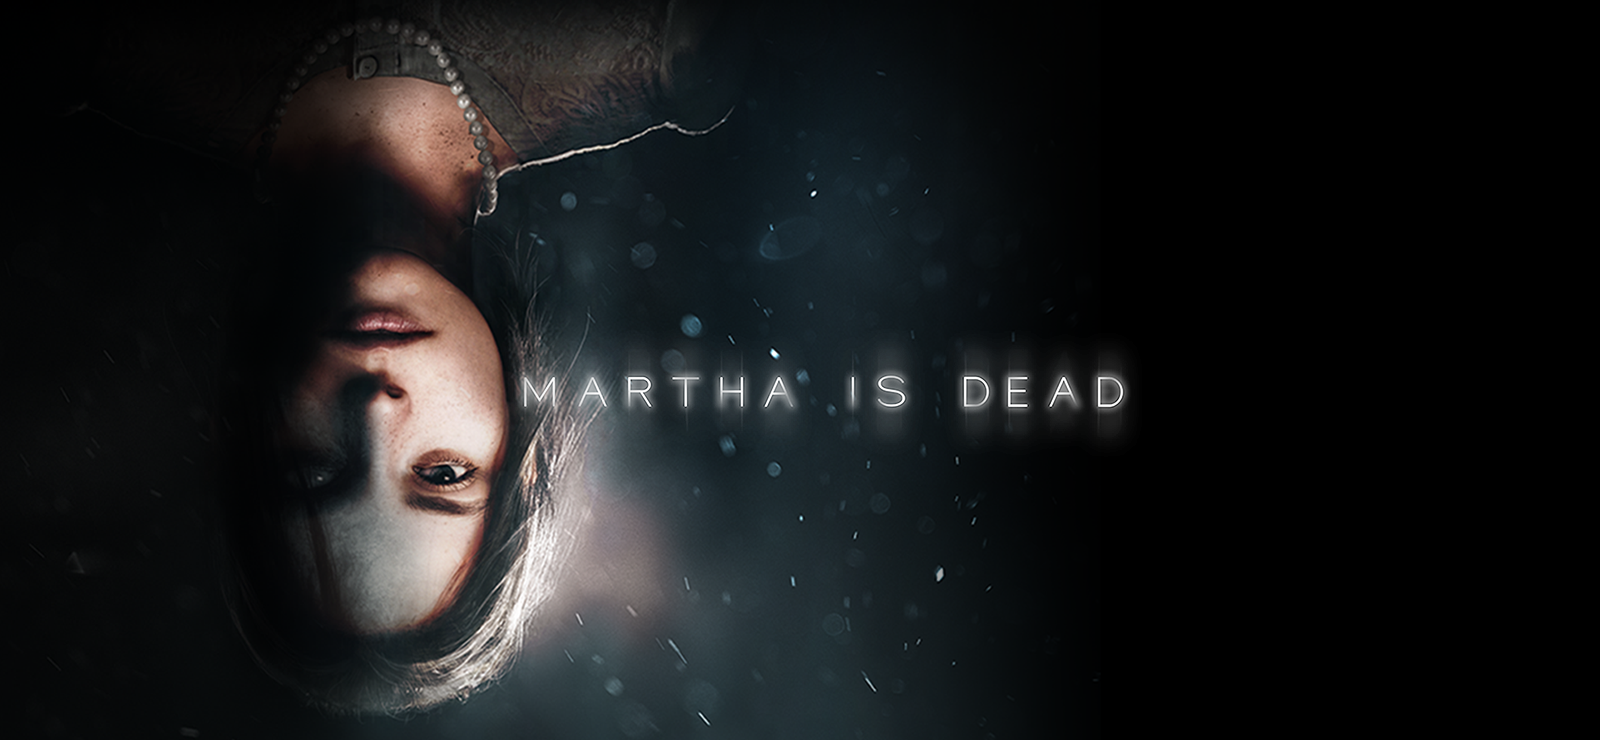
\includegraphics[width=0.6\textwidth, height=0.2\textheight]{Images/martha_is_dead.png}
  \caption{Martha is dead จากเว็บไซต์}\label{martha_is_dead}
\end{figure}
% \subsubsection{Subsubsection 2 heading goes here}
% Subsubsection 2 text

% \subsubsection{Subsubsection 2 heading goes here}
% Subsubsection 2 text

\section{โปรแกรมที่เกี่ยวข้อง}
\subsection{Unity Editor}
\subsubitem \textbf{Unity Editor} \cite{unity:program} เป็นโปรแกรมที่ใช้ในการพัฒนาวอฟต์แวร์และการจำลองต่างๆ เช่น เกม ภาพยนต์ แอนิเมชั่น เป็นต้น ซึ่งใช้ภาษา C$\#$ เป็นหลัก ทั้งนี้ Unity ยังมี Unity asset store พื้นที่ที่ใช้ในการ ซื้อ-ขายชิ้นงาน
\begin{figure}[h]
  \centering
  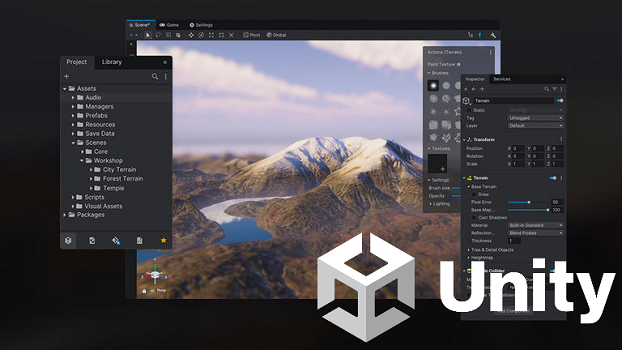
\includegraphics[width=0.6\textwidth, height=0.2\textheight]{Images/unity-engine-landscape-swimlane.png}
  \caption{Unity Editor จากเว็บไซต์}\label{Unity}
\end{figure}

\subsection{Microsoft Visual Studio}
\subsubitem \textbf{Microsoft Visual Studio} \cite{microsoft-visual-studios:program} เป็น IDE ที่ถูกพัฒนาขึ้นโดย Microsoft เป็นเครื่องมือที่ช่วยนักพัฒนาซอฟต์แวร์พัฒนาโปรแกรมคอมพิวเตอร์ เว็บไซต์ เว็บแอปพลิเคชั่น และเว็บเซอร์วิซ
\begin{figure}[h]
  \centering
  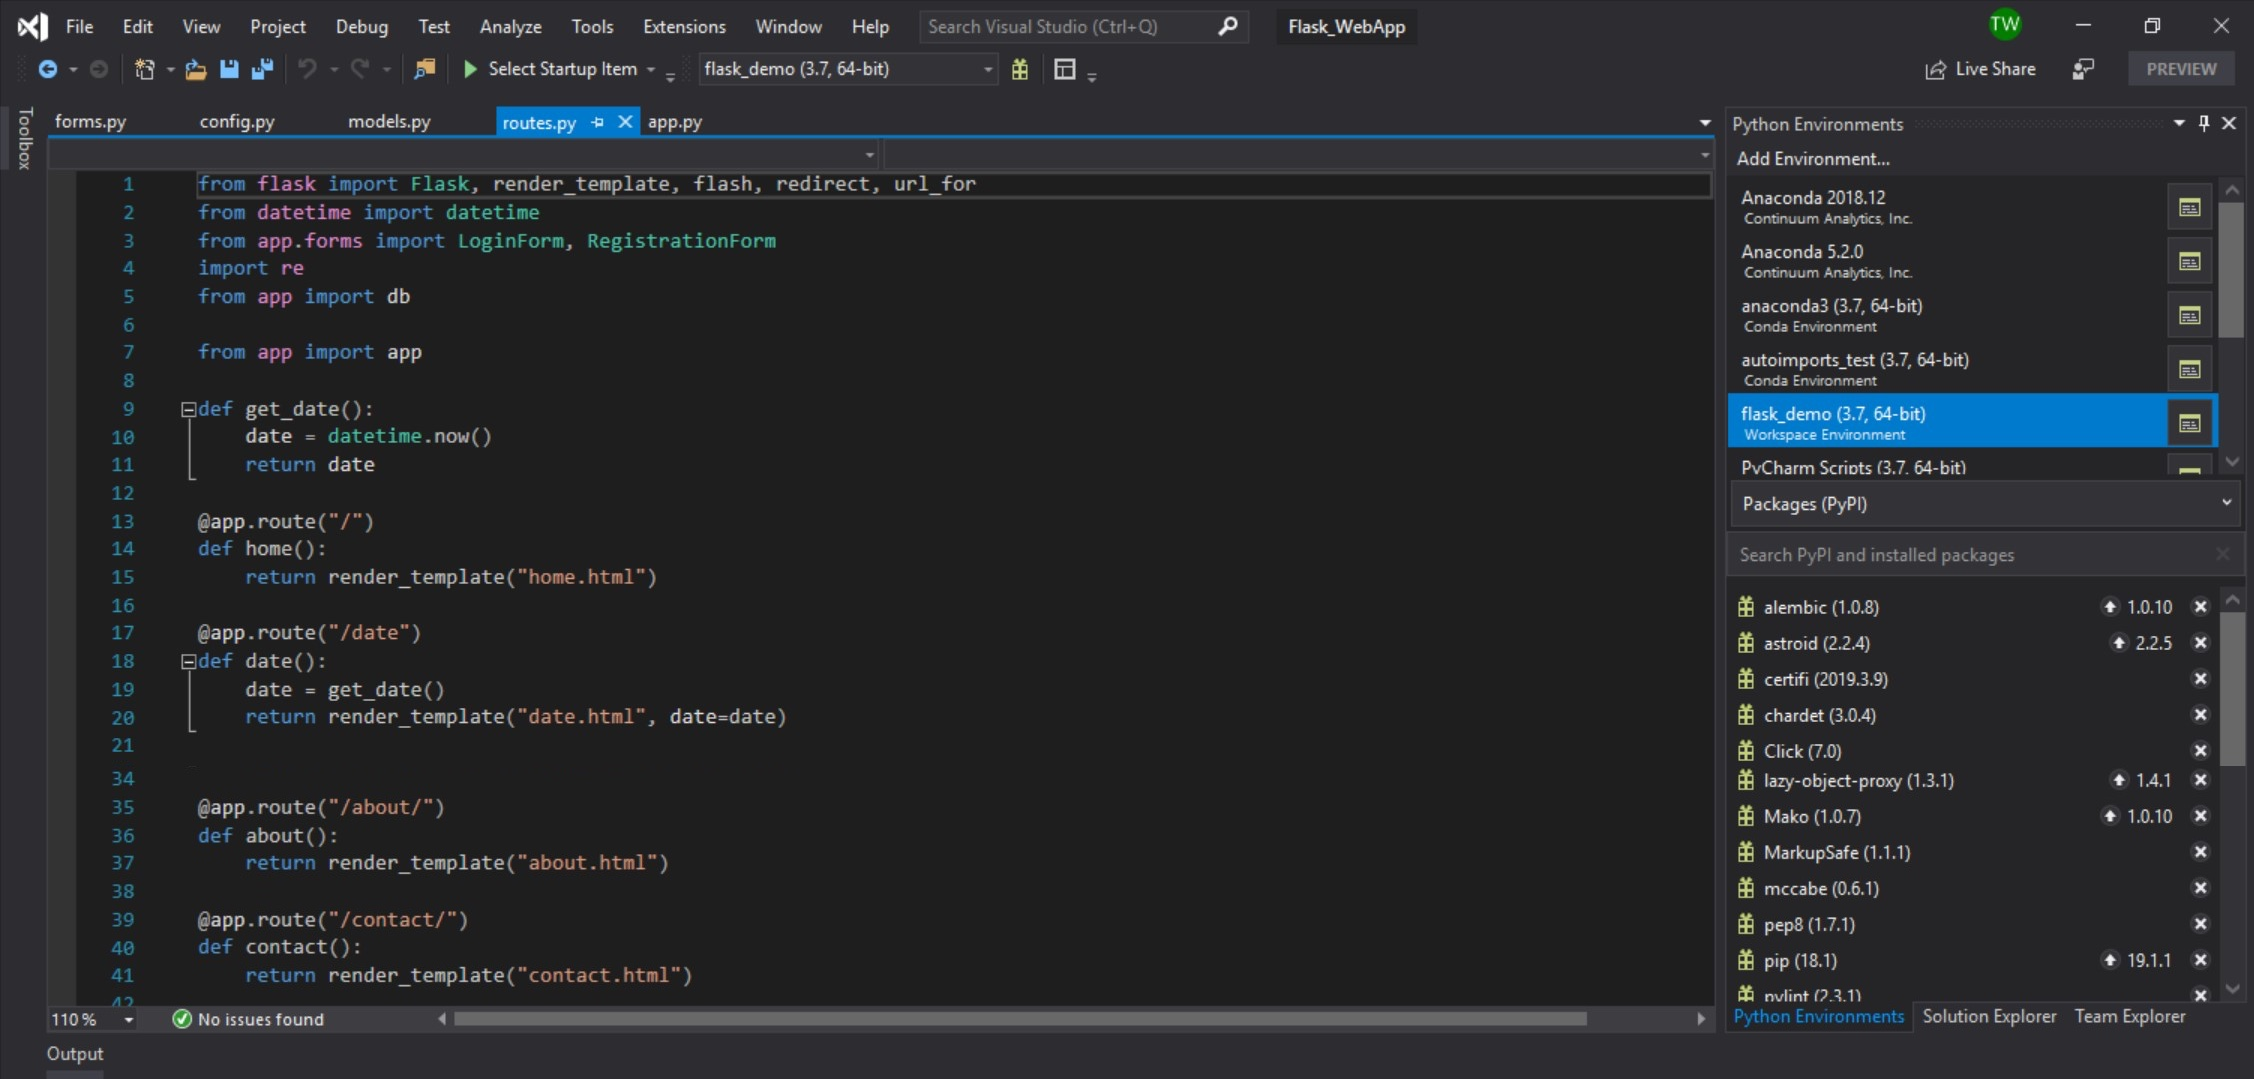
\includegraphics[width=0.6\textwidth, height=0.2\textheight]{Images/python-development-cropped.jpg}
  \caption{Microsoft Visual Studio จากเว็บไซต์}\label{Microsoft}
\end{figure}

\subsection{Jira}
\subsubitem \textbf{Jira} \cite{jira:program} เป็นแอปพลิเคชั่นที่พัฒนาโดย Atlassian ช่วยให้ติดตามความคืบหน้าของงานและจุดบกพร่อง และยังช่วยให้โครงการมีความคล่องตัวมากขึ้น
\begin{figure}[h]
  \centering
  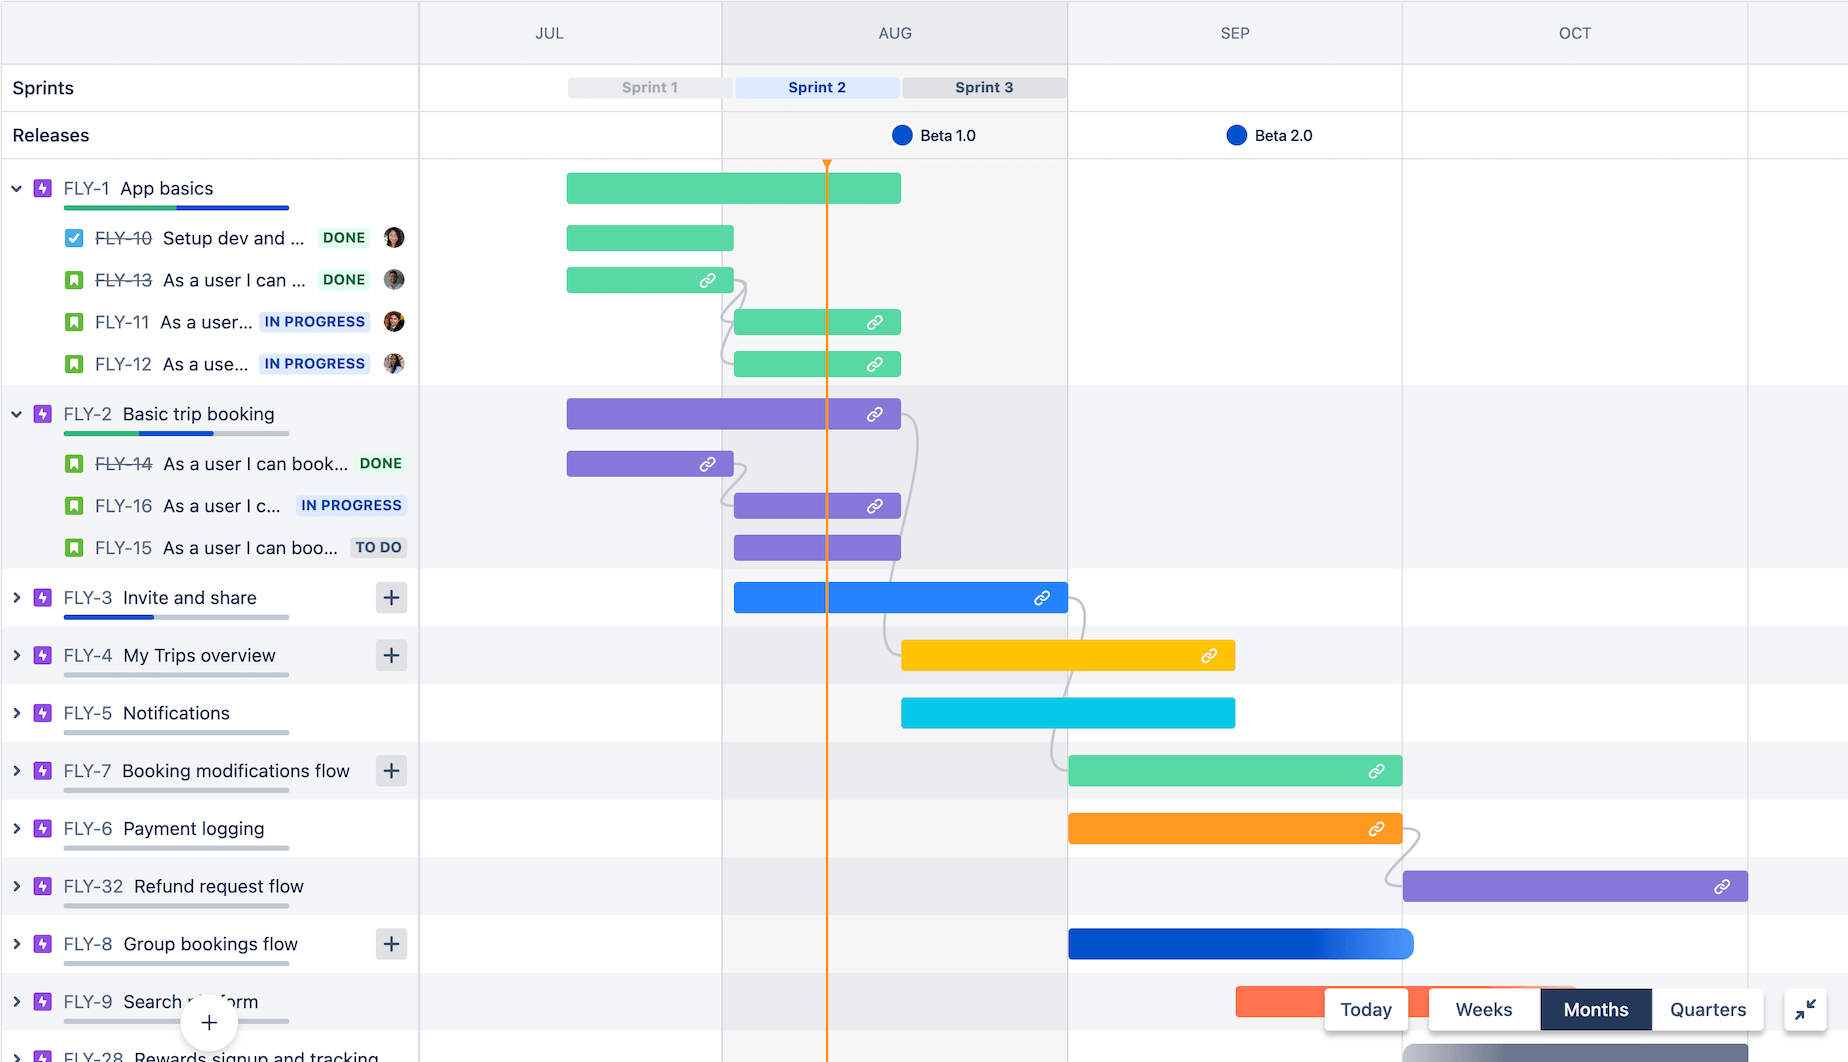
\includegraphics[width=0.6\textwidth, height=0.2\textheight]{Images/screen-roadmaps.png}
  \caption{Jira Platform จากเว็บไซต์}
\end{figure}

\subsection{Unity Asset Store}
\textbf{Japanese School - Stylized} \cite{japanese-school:asset} 
ใช้ในการสร้างฉากโรงเรียน โดยนำส่วนประกอบต่างๆ มาประกอบร่างกัน
\begin{figure}[h]
  \centering
  \includegraphics[width=0.6\textwidth, height=0.2\textheight]{Images/c7836435-cb4d-4b89-9620-466dbdd5a403_orig.png}
  \caption{Japanese School - Stylized จากเว็บไซต์}\label{JapaneseSchool}
\end{figure}
\newline
\textbf{Casual 1 - Anime Girl Characters} \cite{anime-girl:asset} 
ใช้เป็น Main Character ในรุ่นทดลอง
\begin{figure}[h]
  \centering
  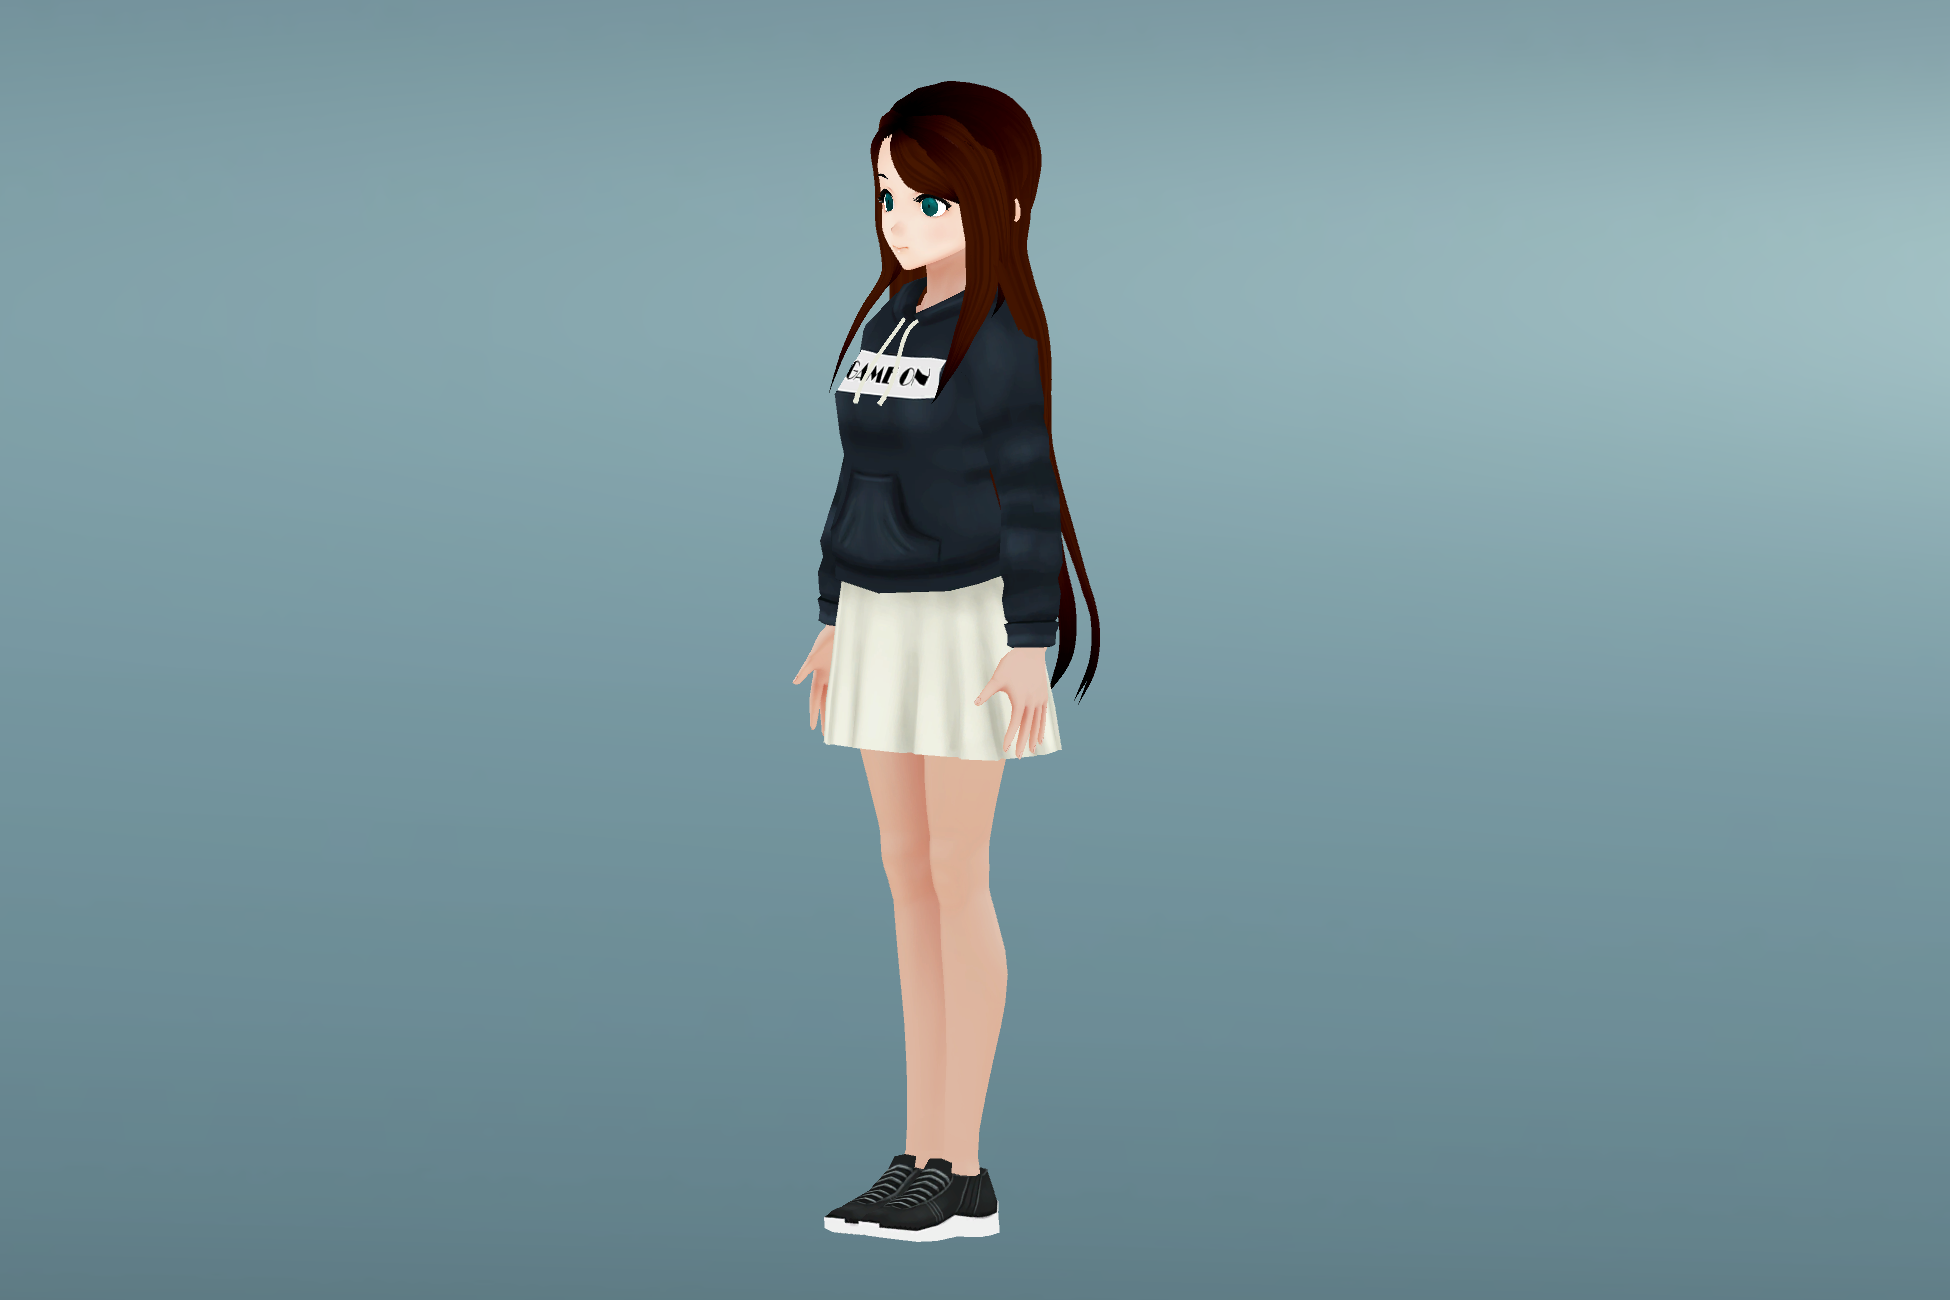
\includegraphics[width=0.6\textwidth, height=0.2\textheight]{Images/7c8d1857-1f28-440d-a966-2c09fe1db214_orig.png}
  \caption{Casual 1 - Anime Girl Characters จากเว็บไซต์}\label{AnimeGirl}
\end{figure}
\newline

% Section 3 text. The dielectric constant\index{dielectric constant}
% at the air-metal interface determines
% the resonance shift\index{resonance shift} as absorption or capture occurs
% is shown in Equation~\eqref{eq:dielectric}:

% \begin{equation}\label{eq:dielectric}
% k_1=\frac{\omega}{c({1/\varepsilon_m + 1/\varepsilon_i})^{1/2}}=k_2=\frac{\omega
% \sin(\theta)\varepsilon_\mathit{air}^{1/2}}{c}
% \end{equation}

% \noindent
% where $\omega$ is the frequency of the plasmon, $c$ is the speed of
% light, $\varepsilon_m$ is the dielectric constant of the metal,
% $\varepsilon_i$ is the dielectric constant of neighboring insulator,
% and $\varepsilon_\mathit{air}$ is the dielectric constant of air.

% \section{About using figures in your report}

% define a command that produces some filler text, the lorem ipsum.
\newcommand{\loremipsum}{
  \textit{Lorem ipsum dolor sit amet, consectetur adipisicing elit, sed do
    eiusmod tempor incididunt ut labore et dolore magna aliqua. Ut enim ad
    minim veniam, quis nostrud exercitation ullamco laboris nisi ut
    aliquip ex ea commodo consequat. Duis aute irure dolor in
    reprehenderit in voluptate velit esse cillum dolore eu fugiat nulla
    pariatur. Excepteur sint occaecat cupidatat non proident, sunt in
    culpa qui officia deserunt mollit anim id est laborum.}\par}

% \begin{figure}
%   \centering

%   \fbox{
%      \parbox{.6\textwidth}{\loremipsum}
%   }

%   % To include an image in the figure, say myimage.pdf, you could use
%   % the following code. Look up the documentation for the package
%   % graphicx for more information.
%   % \includegraphics[width=\textwidth]{myimage}

%   \caption[Sample figure]{This figure is a sample containing \gls{lorem ipsum},
%   showing you how you can include figures and glossary in your report.
%   You can specify a shorter caption that will appear in the List of Figures.}
%   \label{fig:sample-figure}
% \end{figure}

% Using \verb.\label. and \verb.\ref. commands allows us to refer to
% figures easily. If we can refer to Figures
% \ref{fig:walrus} and \ref{fig:sample-figure} by name in the {\LaTeX}
% source code, then we will not need to update the code that refers to it
% even if the placement or ordering of the figures changes.

% \loremipsum\loremipsum

% This code demonstrates how to get a landscape table or figure. It
% uses the package lscape to turn everything but the page number into
% landscape orientation. Everything should be included within an
% \afterpage{ .... } to avoid causing a page break too early.
% \afterpage{
%   \begin{landscape}
%   \begin{table}
%     \caption{Sample landscape table}
%     \label{tab:sample-table}

%     \centering

%     \begin{tabular}{c||c|c}
%         Year & A & B \\
%         \hline\hline
%         1989 & 12 & 23 \\
%         1990 & 4 & 9 \\
%         1991 & 3 & 6 \\
%     \end{tabular}
%   \end{table}
%   \end{landscape}
% }

% \loremipsum\loremipsum\loremipsum

% \section{Overfull hbox}

% When the \verb.semifinal. option is passed to the \verb.cpecmu. document class,
% any line that is longer than the line width, i.e., an overfull hbox, will be
% highlighted with a black solid rule:
% \begin{center}
% \begin{minipage}{2em}
% juxtaposition
% \end{minipage}
% \end{center}
\section{\ifenglish%
    \ifcpe CPE \else ISNE \fi knowledge used, applied, or integrated in this project
  \else%
    ความรู้ตามหลักสูตรซึ่งถูกนำมาใช้หรือบูรณาการในโครงงาน
  \fi
 }

% อธิบายถึงความรู้ และแนวทางการนำความรู้ต่างๆ ที่ได้เรียนตามหลักสูตร ซึ่งถูกนำมาใช้ในโครงงาน
\begin{itemize}
  \item \textbf{Object-Oriented programming} ออกแบบโครงสร้างหลักของการเขียนโปรแกรม การตั้งค่าองค์ประกอบต่างๆ และการเขียนโปรแกรมเชิงวัตถุ
  \item \textbf{Algorithms} ใช้ในการออกแบบ logic เพื่อเพิ่มประสิทธิภาพในการทำงานหรือการคำนวนของ function
  \item \textbf{Software Engineering} ใช้หลักการการพัฒนาซอฟต์แวร์อย่างเป็นระบบ ในการพัฒนาเกมขึ้นมา
  \item \textbf{HCI} ใช้ในการปรับปรุงหน้าตาของระบบเพื่อให้ ผู้เล่นเข้าใจได้ง่าย
\end{itemize}

\section{\ifenglish%
    Extracurricular knowledge used, applied, or integrated in this project
  \else%
    ความรู้นอกหลักสูตรซึ่งถูกนำมาใช้หรือบูรณาการในโครงงาน
  \fi
 }

% อธิบายถึงความรู้ต่างๆ ที่เรียนรู้ด้วยตนเอง และแนวทางการนำความรู้เหล่านั้นมาใช้ในโครงงาน
\begin{itemize}
  \item \textbf{Unity Library} เรียนรู้การใช้งาน Unity และการทำงานของตัว library เป็นหัวใจหลักในการใช้องค์ความรู้จากการศึกษามาพัฒนาเกม
  \item \textbf{Game Design} เรียนรู้การออกแบบระบบให้กับการพัฒนาเกมให้มีความสมบูรณ์
  \item \textbf{Graphics Design} เรียนรู้การออกแบบและจัดวางองค์ประกอบ เพื่อที่จะนำไปใช้ในการออกแบบองกค์ประกอบของภาพ และความกลมกลืน
\end{itemize}

\chapter{\ifproject%
      \ifenglish Project Structure and Methodology\else โครงสร้างและขั้นตอนการทำงาน\fi
  \else%
      \ifenglish Project Structure\else โครงสร้างของโครงงาน\fi
  \fi
 }



\makeatletter

% \renewcommand\section{\@startsection {section}{1}{\z@}%
%                                    {13.5ex \@plus -1ex \@minus -.2ex}%
%                                    {2.3ex \@plus.2ex}%
%                                    {\normalfont\large\bfseries}}

\makeatother
%\vspace{2ex}
% \titleformat{\section}{\normalfont\bfseries}{\thesection}{1em}{}
% \titlespacing*{\section}{0pt}{10ex}{0pt}

\section{\ifenglish Story line\else ภาพรวมของเกม\fi }
เป็นเกมที่จะมีเรื่องราวให้ผู้เล่นได้สวมบทบาทและเผชิญหน้ากับสิ่งที่น่าหวาดกลัว ความกดดัน และเอาตัวรอดจากสถานการณ์ต่าง ๆ ในเกม ซึ่งเป็นแนวเกมที่ได้รับความนิยมในยุคปัจจุบัน โดยในโครงงานนี้ จะเป็นการพัฒนาเกมแนวสยองขวัญ ที่มีมุมมองบุคคลที่ 3 แบบด้านข้าง โดยผู้เล่นจะได้รับบทบาทเป็นนักเรียนคนหนึ่ง ที่มีเพื่อนสนิทพยายามฆ่าตัวตาย แต่ไม่สำเร็จ และนอนไม่ได้สติอยู่ในโรงพยาบาล ผู้เล่นจะต้องค้นหาความจริง โดยการไขปริศนาต่าง ๆ และต้องเอาตัวรอดจากอุปสรรคที่คอยรบกวนผู้เล่น ไม่ให้ไปถึงความจริง และต้องการจะปลิดชีพผู้เล่น ระบบของเกมจะถูกออกแบบให้ผู้เล่นจะต้องคอยบริหารค่าพลังงานที่ใช้ในการทำกิจกรรมต่างๆ ค่าสติที่มีผลกับการรับรู้ของตัวละคร และเวลาที่มีอยู่อย่างจำกัด ซึ่งข้อจำกัดเหล่านี้จะส่งผลให้ผู้เล่นมีความกดดันในการตัดสินใจเลือกการกระทำ สำหรับการดำเนินเนื้อเรื่องและฉากจบ จะมีการเปลี่ยนแปลงไปตามการเลือก ข้อมูล และไอเทมที่ได้รับในระหว่างเล่นเกม


% \section{\ifenglish Work flow game\else ลำดับการทำงาน\fi}
% \begin{figure}[h]
%     \centering
%     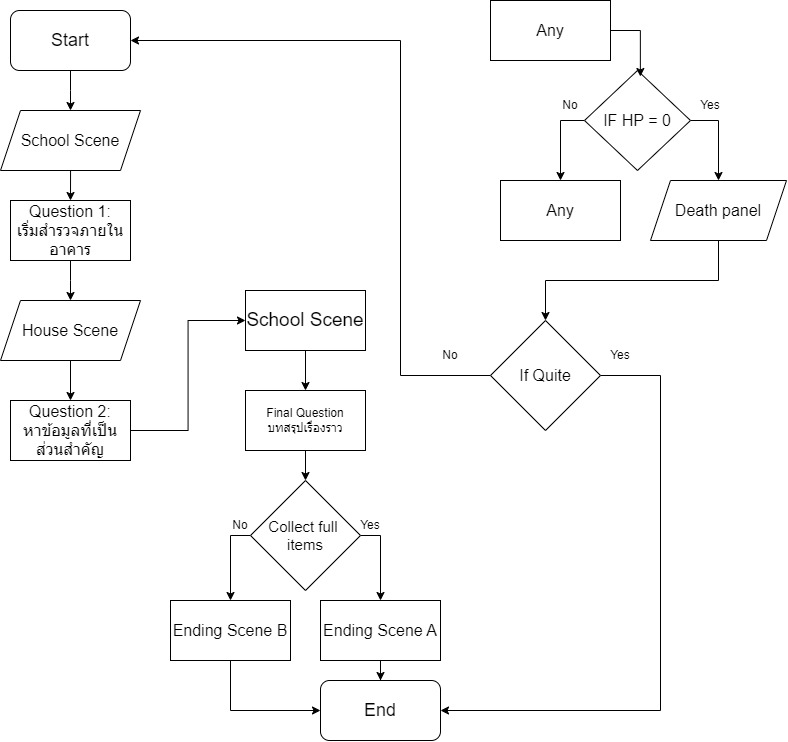
\includegraphics[width=\textwidth, height=0.5\textheight]{Images/FlowChart.jpg}
% \end{figure}

\section{\ifenglish Story board\else เนื้อเรื่องภายในเกม\fi}

\textbf{intro}
เช้าวันหนึ่งที่ไปโรงเรียน มีดอกไม้และข้อความแปลก ๆ วางอยู่บนโต๊ะของเพื่อนสนิท ยังไม่ทันได้หายสงสัย ครู
ประจําชั้นก็เข้ามาในคาบ homeroom และได้พูดขึ้นว่า เพื่อนของเขาหรือแพรวนอนไม่ได้สติอยู่ที่โรงพยาบาล อาการ
สาหัสมาก แต่ไม่ทราบสาเหตุ ทําให้เขานั้นไม่เชื่อและเกิดความคิดที่อยากจะหาความจริงเกี่ยวกับเรื่องนี้ เลยมุ่งหน้าไปที่โรงพยาบาล และแอบเข้าไปดูแพรวในห้องพักผู้ป่วยฉุกเฉิน โดยการหลอกกดปุ่มสัญญาณเตือนไฟไหม้ ทำให้พยาบาลต่างก็วิ่งหนีออกมา ในขณะนั้นเขาจึงเข้าไปที่เคาท์เตอร์พยาบาลเพื่อทำการค้นหาชื่อแพรวและเลขเตียง จากนั้นเขาจึงออกตามหาตามห้องที่ได้บอกไว้ จึงได้พบว่าสิ่งที่ครูประจําชั้นพูดนั้นเป็นความจริง หลังจากนั้นเราก็ได้เดินออกมาจากห้องพักผู้ป่วยด้วยความรู้สึกสงสัยปนเศร้า ทันใดนั้นก็มีแสงวาบเกิดขึ้น และตัวเขาก็ได้ย้อนไปในอดีตเพื่อรับรู้และแก้ไขเรื่องราวได้สมใจ โดยเรื่องราวหลังจากย้อนไปในอดีตนั้น จะย้อนเวลาไป 1 วันก่อนที่แพรวจะลงมือฆ่าตัวตาย โดยเริ่มจากที่บ้าน
 
\textbf{chapter1}
ซึ่งเหตุการณ์ภายในบ้านนั้นจะมีฉากการทะเลาะกับของแพรวกับแม่ และ มีการทำร้ายร่างกาย ด่าทอกันเกิดขึ้น เพราะแม่ไม่พอใจที่เพื่อนมีผลการเรียนที่ไม่ดี ถึงแม้วิชานั้นแพรวจะพยายามถึงที่สุดแล้วก็ตาม
พอทะเลาะกันเสร็จแม่จะเดินออกจากห้องของแพรว และเราก็เดินเข้าไปหาแพรวเพื่อปลอบโยน แต่พูดไปเท่าไรก็เหมือนจะไม่ได้ยินเพราะเธอกำลังร้องไห้อยู่ เลยทำได้แค่กอดเพื่อนไว้ หลังจากนั้นเราสามารถสำรวจห้องนอนของแพรวได้โดยการเดินไปรอบๆห้อง และเก็บของที่พอจะดูเป็นสาเหตุที่ทำให้แพรวเป็นแบบนั้น เช่นใบเกรดที่ถูกฉีกเนื่องจากการทะเลาะกับแม่เมื่อสักครู่ และเมื่อเราเดินออกจากห้องนอนของแพรวเพื่อจะกลับบ้าน กลับพบว่ามีวิญญาณร้ายกำลังเดินตามมาทำร้าย ทำให้ต้องหลบซ่อนโดยแอบในห้องน้ำ และพยายามทำทุกวิถีทางไม่ให้วิญญาณร้ายเปิดประตูได้ และหลังจากนั้นเราจะได้เบาะแสเพิ่มเติมจากวิญญาณ ก่อนที่จะหายไป 

\textbf{chapter2}
ต่อมาจะเป็นฉากในโรงเรียน ซึ่งแพรวก็ยังมาโรงเรียนตามปกติ ในสภาพยิ้มแย้มแจ่มใสเหมือนที่เคยเป็น แต่แล้วตอนคาบพักของวิชาหนึ่ง ได้มีเพื่อนที่ไม่ค่อยถูกกับแพรว มาแฉข่าวลือเรื่องคลิปหลุดระหว่างแพรวกับแฟนเก่าที่เพิ่งเลิกกันไปซึ่งเป็นแฟนปัจจุบันของเพื่อนคนนั้น แต่จริง ๆ แล้วในคลิปนั้นเป็นแค่คนหน้าเหมือนกันเท่านั้น แต่ทุกคนในห้องก็ตราหน้าเธอไปแล้วว่าเป็นนักเรียนที่ไม่ดี อีกทั้งแฟนเก่าของเธอก็ยังเพิกเฉยต่อข่าวข่าวนี้ ซึ่งในขณะนั้นเราก็สังเกตเห็นได้ว่า ตัวเราเองในอดีตนั้น ไม่ได้ออกมาปกป้องเพื่อนเลยแม้แต่น้อยเพราะกลัวว่าจะโดนลูกหลงไปด้วย เราเลยเริ่มเอะใจแล้วว่า หรือจริง ๆ แล้ว นี่ไม่ใช่การแก้ไขอดีต แต่เป็นการย้อนเวลามาดูอดีตต่างหาก อย่างไรก็ตาม หลังจากที่แพรวโดนตราหน้าไปแบบนั้น เธอจึงวิ่งหนีออกไปที่ห้องน้ำ เราจึงตามไปดูว่าแพรวไปที่ไหน ระหว่างที่เธอกำลังตามไปดู จู่ ๆ เราก็มีอาการคล้าย ๆ กับหน้ามืด และวิญญาณตัวนั้นก็โผล่มาอีกครั้ง ทำให้เราต้องวิ่งหนีเข้าห้องน้ำ และป้องกันไม่ให้วิญญาณร้ายเปิดประตูได้ แต่ครั้งนี้กลับไม่สำเร็จจึงโดนทำร้าย และก่อนที่วิญญาณจะจากไปมันได้บอกว่า"วันนี้ หัวค่ำ ดาดฟ้า" ซึ่งอาจจะเป็นเบาะแสอะไรบางอย่าง หลังจากวิญญาณหายไป เราก็ตามหาแพรวจากเสียงสะอื้นในห้องน้ำอีกครั้ง และพยายามเคาะประตู แต่ก็ไม่เป็นผล เพราะเหมือนเธอไม่ได้ยินอะไรเลย ทำให้เราต้องเดินออกมา ระหว่างที่เดินกลับไปที่ห้องเรียน เราก็ได้ยินผู้คนพูดถึงเรื่องคลิปหลุดของแพรว ทำให้เธอรู้ว่าข่าวลือนั้นได้สะพัดไปทั่วโรงเรียนแล้ว
เย็นวันนั้น แพรวไม่ยอมกลับบ้าน เพราะเธอกลัวว่าจะโดนแม่ของเธอต่อว่าอีก และเธอต้องการจะเคลียร์กับแฟนเก่าว่าทำไมถึงเกิดเรื่องแบบนี้ขึ้นกับเธอ แต่เธอก็โดนเขาต่อว่าอีกว่าเป็นคนไม่สวย เรียนก็ไม่เก่ง ใครจะอยากได้เป็นแฟน และที่ยอมคบกับอีกคนเพราะว่าจริง ๆ เขาได้แอบชอบผู้หญิงคนนั้นมานานแล้ว แต่เธอไม่ยอมรับรักสักที และรู้มาว่าเธอไม่ชอบแพรว เลยมาขอเป็นแฟนเพื่อให้เกิดความหึงหวงขึ้นและรับรักเขาในที่สุด ซึ่งมันก็ได้ผล ทำให้แพรวเสียใจมาก ถึงมากที่สุด และที่โดนปล่อยคลิปหลุดเพราะว่าเธอต้องการให้ทุกคนมองว่าแพรวเป็นคนไม่ดี และให้ทุกคนแบนเธอทิ้งไปซะ โทษฐานแย่งแฟนคนอื่น

\textbf{chapter3}
ด้วยความเสียใจแพรวจึงนั่งร้องไห้อยู่คนเดียวสักพักซึ่งมีเรานั่งอยู่ข้าง ๆ สักพักภาพก็มืดดำไป และตัดกลับมาที่เรายังนั่งอยู่ที่เดิม แต่แพรวไม่อยู่แล้ว ซึ่งจะเดินออกจากโรงเรียนก็ไม่ได้ เพราะเป็นเวลาที่ประตูโรงเรียนปิดแล้ว ทำให้เรานึกคำใบที่วิญญาณพูดกับเธอได้ว่า"วันนี้ หัวค่ำ ดาดฟ้า" เราจึงวิ่งเข้าไปในอาคารเรียน แต่อาคารเรียนล็อก ทำให้ต้องไปหากุญแจมาเปิดให้ได้ ซึ่งก็หาเจอแต่นั่นก็ทำให้วิญญาณร้ายปรากฏตัวอีกครั้ง แต่เวลาเหลือไม่มากแล้ว เลยต้องวิ่งขึ้นไปบนดาดฟ้าให้ทันเพื่อไปดูว่าจะเกิดอะไรขึ้นกับแพรว โดยที่ยังมีวิญญาณวิ่งตามหลัง พอขึ้นไปถึงด้านบน เราจึงตะโกนเรียกชื่อเพื่อนของเธอ ทำให้แพรวที่กำลังจะกระโดดลงจากตึกนั้นชะงักและหันมามอง เราจึงเข้าไปจับมือและห้ามไม่ให้เพื่อนกระโดด แต่เธอก็ยังยืนยันที่จะจบชีวิตตัวเอง เธอเกลียดตัวเอง เกลียดมากซะจนอยากจะฆ่ามันทิ้งไปซะ ไม่มีใครรักเธอแล้ว เธอล้มเหลวทุกอย่างในชีวิต ทันใดนั้นวิญญาณร้ายก็ได้โผล่ขึ้นมา ซึ่งเราหมดหนทางหนีแล้ว ทำให้ต้องต่อสู้และระหว่างการต่อสู้นั้นทำให้แพรวเห็นว่า ยังมีคนที่อยู่เคียงข้างมาตลอด แค่ระหว่างทางนั้นเราไม่กล้าที่จะพูดหรือแสดงออกเพราะกลัวสังคมตราหน้า แต่ตอนนี้เธอไม่กลัวอะไรอีกแล้ว ระหว่างที่สู้กับวิญญาณร้ายเราพลาดท่าและตกตึกลงไปแทนแพรว แพรวที่เห็นดังนั้นก็เป็นลมสลบไป และยามที่เห็นว่ามีคนร่วงมาจากดาดฟ้าและเห็นว่ามีคนยืนอยู่ก็ได้ขึ้นมาช่วยแพรวไว้ และแจ้งตำรวจว่ามีนักเรียนตกตึกจึงนำตัวส่งโรงพยาบาลและเสียชีวิตในเวลาต่อมา

\textbf{last chapter}
2สัปดาห์ต่อมา แพรวได้รับความยุติธรรมว่าในคลิปนั้นไม่ใช่เธอ และทางโรงเรียนก็เอาผิดเพื่อนคนนั้นที่ปล่อยข่าวลือโดยการพักการเรียน 1 เทอมการศึกษา ทำให้แพรวได้กลับมาใช้ชีวิตในรั้วโรงเรียนได้อีกครั้ง แต่เธอก็ยังยืนยันว่าจะลาออกจากโรงเรียนที่นี่แล้วย้ายบ้านออกไปอยู่กับพ่อ เนื่องจากเธอได้แจ้งตำรวจไปเมื่อวันที่เธอจะทำการฆ่าตัวตาย ว่าแม่ของเธอมีการใช้กำลังเกิดขึ้น ทำให้เรื่องไปถึงพ่อ พ่อจึงฟ้องหย่ากับภรรยา และขอสิทธิ์เลี้ยงดูลูกทำให้เธอต้องย้ายไปต่างจังหวัดเพื่ออยู่กับพ่อ อย่างไรก็ตามเธอมาโรงเรียนวันสุดท้ายเพื่อเก็บของ และเห็นว่ามีดอกไม้วางอยู่บนโต๊ะ พร้อมข้อความให้กำลังใจเธอเต็มไปหมด เช่น ขอให้เธอปลอดภัย แต่ถัดไปโต๊ะอีกตัว ซึ่งเป็นโต๊ะของเรา ไม่มีแม้แต่เศษกระดาษมาวางไว้ ทั้ง ๆ ที่เราได้ตายไปแล้ว แพรวจึงวางดอกไม้สีขาวไว้บนโต๊ะเรา เพื่อเป็นการไว้อาลัย ก่อนที่เธอจะเดินออกจากห้องไปเพื่อเริ่มต้นชีวิตใหม่


\section{\ifenglish Story line\else องค์ประกอบภายในเกม\fi }
\subsection{\ifenglish Story line\else ตัวละคร\fi }
ในที่นี้ จะแบ่งเป็นตัวละครหลักและตัวละครเสริม
\subitem ตัวละครหลัก
\begin{itemize}
    \item \textbf{ตัวเอก} เป็นนักเรียนหญิงชั้นมัธยมปลาย ผมสั้น สวมใส่แว่น มีลักษณะนิสัย เป็นคนเงียบๆ มีเพื่อนน้อย ไม่ค่อยมีมนุษย์ปฏิสัมพันธ์
    \begin{figure}[h]
        \centering
        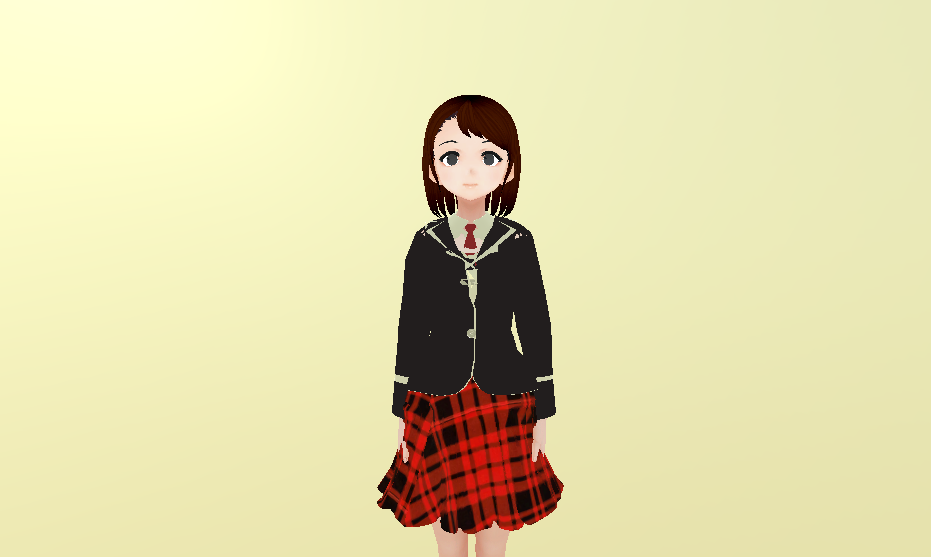
\includegraphics[scale=0.5]{Images/main char image.png}
        \caption{ภาพตัวละครหลัก}\label{MainCharacter}
    \end{figure}
    \item \textbf{แพรว} เป็นนักเรียนหญิงชั้นมัธยมปลาย ผมยาว มีลักษณะนิสัย เป็นคนจริงจังกับทุกๆเรื่อง และต้องการทำทุกๆอย่างให้สมบูรณ์แบบมากที่สุด เพื่อเอาใจคนรอบข้าง
    \begin{figure}[h]
        \centering
        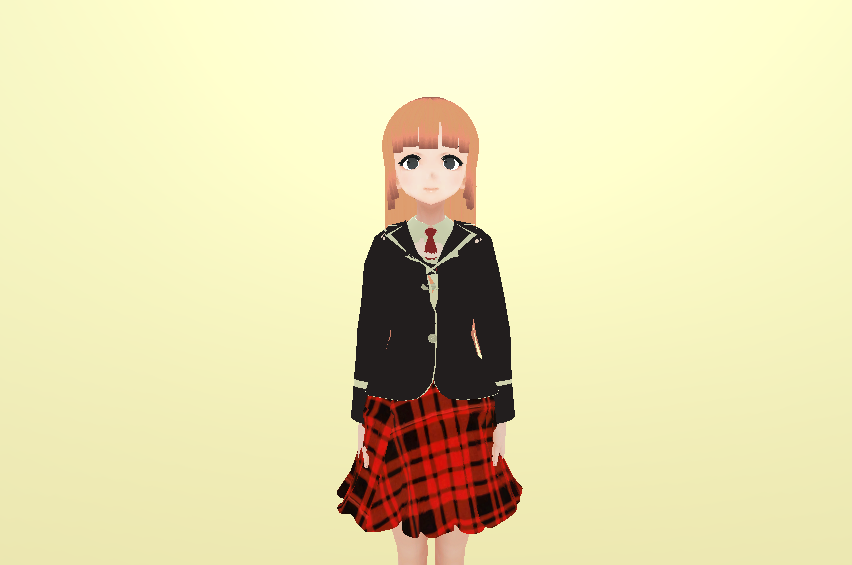
\includegraphics[scale=0.5]{Images/Preaw Image.png}
        \caption{ภาพตัวละครแพรว}\label{PrawCharacter}
    \end{figure}
    \item \textbf{วิญญาณร้าย} ผู้หญิงผมยาวสีดำ ดวงตามีสีดำล้วนเหมือนจะกลวงโบ๋ มีคราบน้ำตาสีเลือดเปื้อนอยู่ที่แก้ม มีลักษณะนิสัย ทุก ๆ ครั้งที่เราจะรู้ความลับของแพรว มันจะปรากฎตัวและทำร้ายเรา ซึ่งเป็นนิสัยอีกด้านของแพรว ที่ไม่ต้องการให้ใครมารับรู้ความลับที่เธอเป็นคนไม่สมบูรณ์แบบ
    \begin{figure}[h]
        \centering
        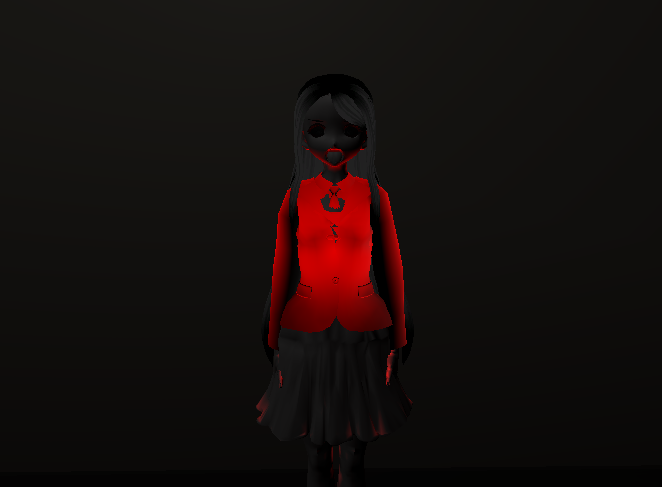
\includegraphics[scale=0.5]{Images/ghost image.png}
        \caption{ภาพตัวละครวิญญาณร้าย}\label{GhostCharacter}
    \end{figure}
\end{itemize}


\subitem ตัวละครเสริม
\begin{itemize}
    \item \textbf{ครูประจำชั้น} เป็นผู้หญิงวัยผู้ใหญ่  ผมยาวประบ่า สวมชุดสุภาพ
    \item \textbf{พยาบาล} เป็นผู้หญิงวัยผู้ใหญ่ เก็บผมเรียบร้อย สวมเครื่องแบบพยาบาล
    \item \textbf{รปภ.} เป็นผู้ชายวัยกลางคน ผมสั้น สวมเครื่องแบบรปภ.
    \item \textbf{นักเรียนหญิง} เป็นผู้หญิงผมยาวประบ่าสีดำ สวมเครื่องแบบนักเรียน
    \item \textbf{นักเรียนชาย} เป็นผู้ชายผมสั้น  สวมเครื่องแบบนักเรียน
    \item \textbf{แม่} เป็นผู้หญิงวัยกลางคน ผมสั้น สวมชุดอยู่บ้าน
\end{itemize}

\subsection{\ifenglish Story line\else ฉาก\fi }
\begin{itemize}
    \item \textbf{โรงเรียน} เป็นอาคาร 3 ชั้น แต่ละชั้นมีห้องเรียน 6 ห้อง มีทั้งห้องเรียน ห้องน้ำ และทางเดินหน้าโรงเรียน
    \item \textbf{โรงพยาบาล} เป็นอาคาร 8 ชั้น ประกอบไปด้วย เคาท์เตอร์พยาบาล และห้องฉุกเฉิน
    \item \textbf{บ้าน} เป็นอาคาร 2 ชั้น ประกอบไปด้วยห้องนอนแพรว
\end{itemize}

\newpage
\subsection{\ifenglish Story line\else การควบคุมตัวละคร\fi }
\begin{center}
    \begin{tabular}{|c|c|}
    \hline
    กดปุ่ม A, D & ใช้ในการเคลื่อนที่ของตัวละครให้เคลื่อนที่ไปทางซ้าย ทางขวา ตามลำดับ\\
    กดปุ่ม W, S ที่บันได& ใช้ในการขึ้นไปข้างบน หรือ ลงข้างล่าง\\
    กดปุ่ม E ที่วัตถุเช่น ประตูหรือกล่อง& ใช้ในการทำการ interaction เปิดประตูหรือเก็บของ\\
    กดปุ่ม E ที่ตู้ล็อคเกอร์หรือห้องน้ำ& เพื่อทำการซ่อนตัวจากศัตรู\\
    ขณะซ่อนตัว กดปุ่ม Q& เพื่อยกเลิกการซ่อนตัว\\
    กดปุ่ม E ค้างที่ กล่องหรือโต๊ะเรียน & ใช้ในการเก็บ/ค้นหา items จากกล่องหรือโต๊ะเรียน\\
    กดปุ่ม I & ใช้ในการเปิด inventory ขึ้นมา\\
    กดปุ่ม Esc& ใช้ในการออกจาก game\\
    หน้า inventory กดที่ item& เพื่อเปิดดูข้อมูลของ items นั้นๆ\\
    หน้า inventory กดปุ่ม use& เพื่อทำการใช้ items นั้นๆ\\
    หน้า inventory กดปุ่ม drop& เพื่อทิ้ง items ที่ไม่ต้องการใช้งาน\\
    หน้า inventory กดปุ่ม กากบาท หรือ ปุ่ม Q& เพื่อปิดหน้า inventory\\
    กดปุ่มลูกศร& เพื่อใช้ในการกด Quick Time Event ที่จะมาในแบบลูกศร\\
    \hline
    \end{tabular}
\end{center}
\subsection{\ifenglish Story line\else ค่าพลัง\fi }
\begin{itemize}
    \item \textbf{ค่าพลังชีวิต} เป็นค่าที่จะส่งผลต่อการมีชีวิตของตัวละคร เป็นค่าที่ผู้เล่นจะต้องประคองไม่ให้หมด จะนำไปสู่ Game over
    \item \textbf{ค่าพลังกาย} เป็นค่าที่จะใช้ในการกระทำต่างๆ ทั้ง วิ่งและกระโดด
    \item \textbf{ค่าสติ} เป็นค่าที่จะกำหนดขอบเขตการมองเห็นของผู้เล่น เมื่อมีน้อย มุมมองการมองเห็นจะลดลง
\end{itemize}
\subsection{\ifenglish Story line\else Puzzle\fi }
ภายในเกมจะมี puzzle อยู่ 2 รูปแบบ
\begin{itemize}
    \item การใส่ตัวเลขให้ถูกต้องเพื่อชนะปริศนา
    \begin{figure}[h]
        \centering
        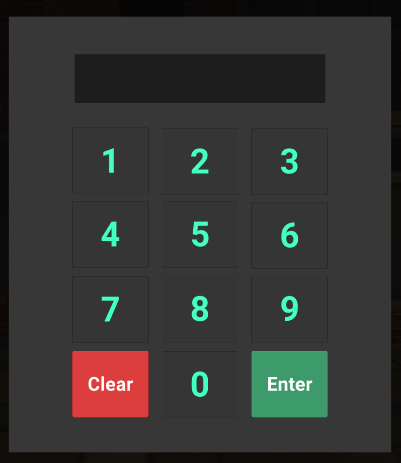
\includegraphics[scale=0.5]{Images/Password Image.png}
        \caption{รูปแสดง Puzzle แบบรหัสผ่าน}
    \end{figure}
    \item การกดตามปุ่มที่เกิดขึ้นที่หน้าจอให้ทันตามเวลาที่กำหนด
    \begin{figure}[h]
        \centering
        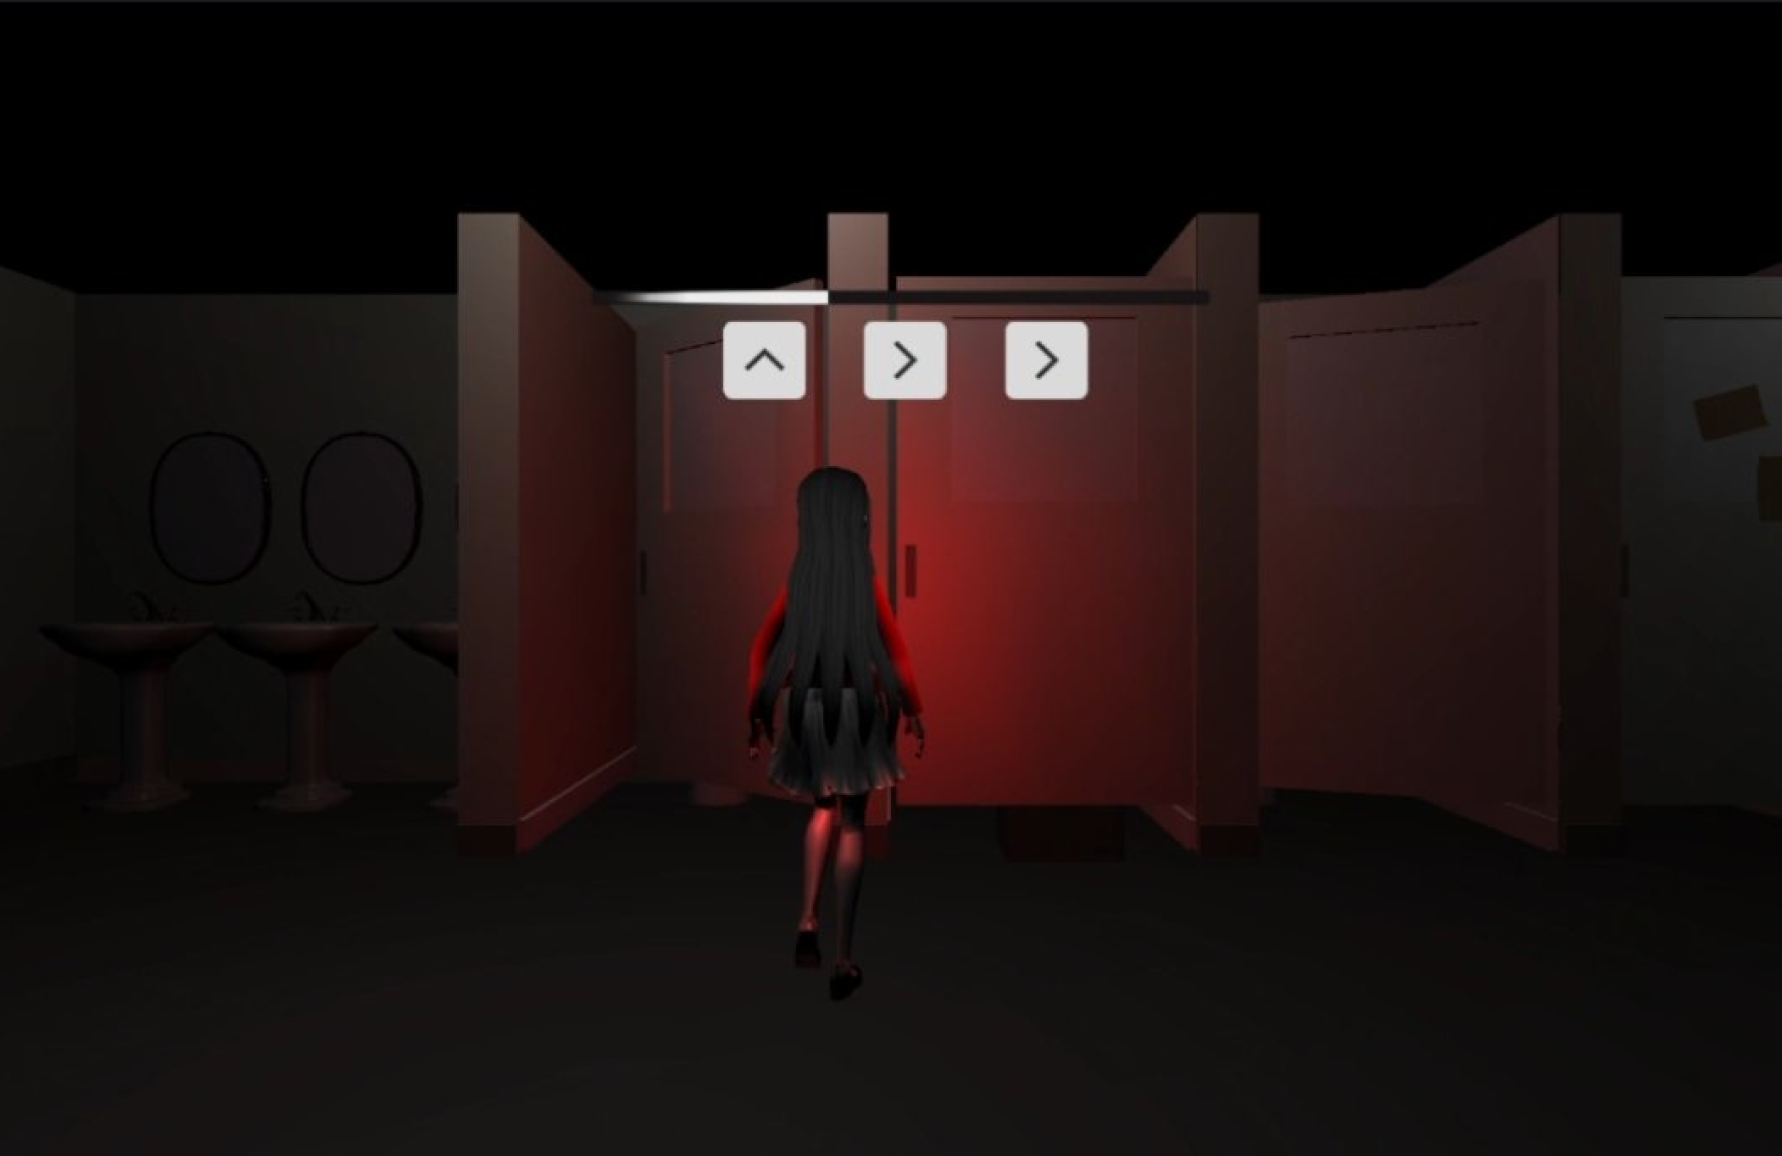
\includegraphics[scale=0.15]{Images/tutorial_qte.png}
        \caption{รูปแสดง Quick Time Event}
    \end{figure}
\end{itemize}
\subsection{\ifenglish Story line\else Item\fi }
\begin{center}
    \begin{tabular}{|c|c|}
    \hline
    อาหารกระป๋อง & เมื่อใช้งาน จะฟื้นฟูค่าพลังชีวิต 25 หน่วย\\
    น้ำดื่ม & เมื่อใช้งาน จะฟื้นฟูค้าพลังชีวิต 10 หน่วย\\
    ชุดปฐมพยาบาล & เมื่อใช้งาน จะฟื้นฟูค้าพลังชีวิต 75 หน่วย\\
    ยาประหลาด & เมื่อใช้งาน จะฟื้นฟูค่าสติ 75 หน่วย\\
    \hline
    \end{tabular}
\end{center}
\subsection{\ifenglish Story line\else ฉากจบ\fi }
มีทั้งหมด 3 ฉากด้วยกัน
\begin{itemize}
    \item \textbf{Good end} จะเกิดขึ้นก็ต่อเมื่อดำเนินเรื่องราวทุกอย่างตามเนื้อเรื่อง และ ขึ้นไปช่วยแพรวจากวิญญาณร้ายได้สำเร็จ กล่าวคือคนที่ตายไปจะมีแค่เราคนเดียว
    \item \textbf{Bad end} จะเกิดขึ้นก็ต่อเมื่อดำเนินเรื่องราวทุกอย่างตามเนื้อเรื่อง แต่ขึ้นไปช่วยแพรวไม่ทันเวลา ทำให้เธอได้กระโดดลงมาก่อน หรือไม่ยอมเรียกชื่อแพรวตอนที่เธอกำลังจะกระโดดลงไป หลังจากนั้น วิญญาณร้ายจะผลักเราตกลงจากตึกด้วยเช่นกัน
    \item \textbf{Game Over} จะเกิดขึ้นก็ต่อเมื่อผู้เล่นโดนวิญญาณร้ายโจมตีจนค่าพลังชีวิตหมด และ เมื่อเกิดฉากจบนี้ เกมจะให้เริ่มเล่นใหม่ ณ chapter นั้นๆ
\end{itemize}
% \begin{figure}
% \begin{center}
% 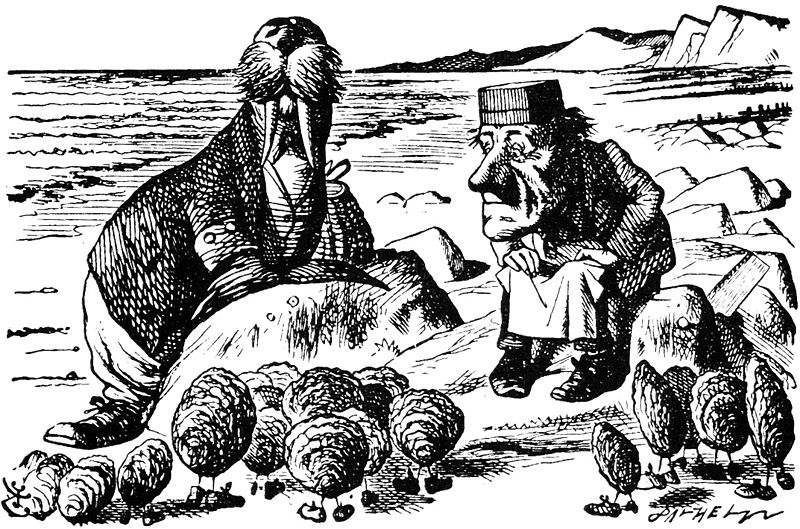
\includegraphics{800px-Briny_Beach.jpg}
% \end{center}
% \caption[Poem]{The Walrus and the Carpenter}
% \label{fig:walrus}
% \end{figure}

% \subsection{The Black Kitten}
%   One thing was certain, that the WHITE kitten had had nothing to
% do with it:---it was the black kitten's fault entirely~\cite{aiw}.  For the
% white kitten had been having its face washed by the old cat for
% the last quarter of an hour (and bearing it pretty well,
% considering); so you see that it COULDN'T have had any hand in
% the mischief.

%   The way Dinah washed her children's faces was this:  first she
% held the poor thing down by its ear with one paw, and then with
% the other paw she rubbed its face all over, the wrong way,
% beginning at the nose:  and just now, as I said, she was hard at
% work on the white kitten, which was lying quite still and trying
% to purr---no doubt feeling that it was all meant for its good.

%   But the black kitten had been finished with earlier in the
% afternoon, and so, while Alice was sitting curled up in a corner
% of the great arm-chair, half talking to herself and half asleep,
% the kitten had been having a grand game of romps with the ball of
% worsted Alice had been trying to wind up, and had been rolling it
% up and down till it had all come undone again; and there it was,
% spread over the hearth-rug, all knots and tangles, with the
% kitten running after its own tail in the middle.

% \subsection{The Reproach}

%   `Oh, you wicked little thing!' cried Alice, catching up the
% kitten, and giving it a little kiss to make it understand that it
% was in disgrace.  `Really, Dinah ought to have taught you better
% manners!  You OUGHT, Dinah, you know you ought!' she added,
% looking reproachfully at the old cat, and speaking in as cross a
% voice as she could manage---and then she scrambled back into the
% arm-chair, taking the kitten and the worsted with her, and began
% winding up the ball again.  But she didn't get on very fast, as
% she was talking all the time, sometimes to the kitten, and
% sometimes to herself.  Kitty sat very demurely on her knee,
% pretending to watch the progress of the winding, and now and then
% putting out one paw and gently touching the ball, as if it would
% be glad to help, if it might.

%   `Do you know what to-morrow is, Kitty?' Alice began.  `You'd
% have guessed if you'd been up in the window with me---only Dinah
% was making you tidy, so you couldn't.  I was watching the boys
% getting in stick for the bonfire---and it wants plenty of
% sticks, Kitty!  Only it got so cold, and it snowed so, they had
% to leave off.  Never mind, Kitty, we'll go and see the bonfire
% to-morrow.'  Here Alice wound two or three turns of the worsted
% round the kitten's neck, just to see how it would look:  this led
% to a scramble, in which the ball rolled down upon the floor, and
% yards and yards of it got unwound again.

%   `Do you know, I was so angry, Kitty,' Alice went on as soon as
% they were comfortably settled again, `when I saw all the mischief
% you had been doing, I was very nearly opening the window, and
% putting you out into the snow!  And you'd have deserved it, you
% little mischievous darling!  What have you got to say for
% yourself?  Now don't interrupt me!' she went on, holding up one
% finger.  `I'm going to tell you all your faults.  Number one:
% you squeaked twice while Dinah was washing your face this
% morning.  Now you can't deny it, Kitty:  I heard you!  What that
% you say?' (pretending that the kitten was speaking.)  `Her paw
% went into your eye?  Well, that's YOUR fault, for keeping your
% eyes open---if you'd shut them tight up, it wouldn't have
% happened.  Now don't make any more excuses, but listen!  Number
% two:  you pulled Snowdrop away by the tail just as I had put down
% the saucer of milk before her!  What, you were thirsty, were you?

\chapter{\ifproject%
\ifenglish Experimentation and Results\else การทดลองและผลลัพธ์\fi
\else%
\ifenglish System Evaluation\else การประเมินระบบ\fi
\fi}

ในบทนี้จะทดสอบเกี่ยวกับการทำงานในฟังก์ชันหลักๆ

\ifproject
  \chapter{\ifenglish Conclusions and Discussions\else บทสรุปและข้อเสนอแนะ\fi}

\section{\ifenglish Conclusions\else สรุปผล\fi}

นศ. ควรสรุปถึงข้อจำกัดของระบบในด้านต่างๆ ที่ระบบมีในเนื้อหาส่วนนี้ด้วย

\section{\ifenglish Challenges\else ปัญหาที่พบและแนวทางการแก้ไข\fi}

ในการทำโครงงานนี้ พบว่าเกิดปัญหาหลักๆ ดังนี้

\section{\ifenglish%
Suggestions and further improvements
\else%
ข้อเสนอแนะและแนวทางการพัฒนาต่อ
\fi
}

ข้อเสนอแนะเพื่อพัฒนาโครงงานนี้ต่อไป มีดังนี้

\fi

\bibliography{sampleReport}

\ifproject
  \normalspacing
  \appendix
  \chapter{The first appendix}

Text for the first appendix goes here.

\section{Appendix section}

Text for a section in the first appendix goes here.

test ทดสอบฟอนต์ serif ภาษาไทย

\textsf{test ทดสอบฟอนต์ sans serif ภาษาไทย}

\verb+test ทดสอบฟอนต์ teletype ภาษาไทย+

\texttt{test ทดสอบฟอนต์ teletype ภาษาไทย}

\textbf{ตัวหนา serif ภาษาไทย \textsf{sans serif ภาษาไทย} \texttt{teletype ภาษาไทย}}

\textit{ตัวเอียง serif ภาษาไทย \textsf{sans serif ภาษาไทย} \texttt{teletype ภาษาไทย}}

\textbf{\textit{ตัวหนาเอียง serif ภาษาไทย \textsf{sans serif ภาษาไทย} \texttt{teletype ภาษาไทย}}}

\url{https://www.example.com/test_ทดสอบ_url}

\chapter{\ifenglish Manual\else คู่มือการใช้งานระบบ\fi}

Manual goes here.


  %% Display glossary (optional) -- need glossary option.
  \ifglossary\glossarypage\fi

  %% Display index (optional) -- need idx option.
  \ifindex\indexpage\fi

  \begin{biosketch}
    \begin{center}
      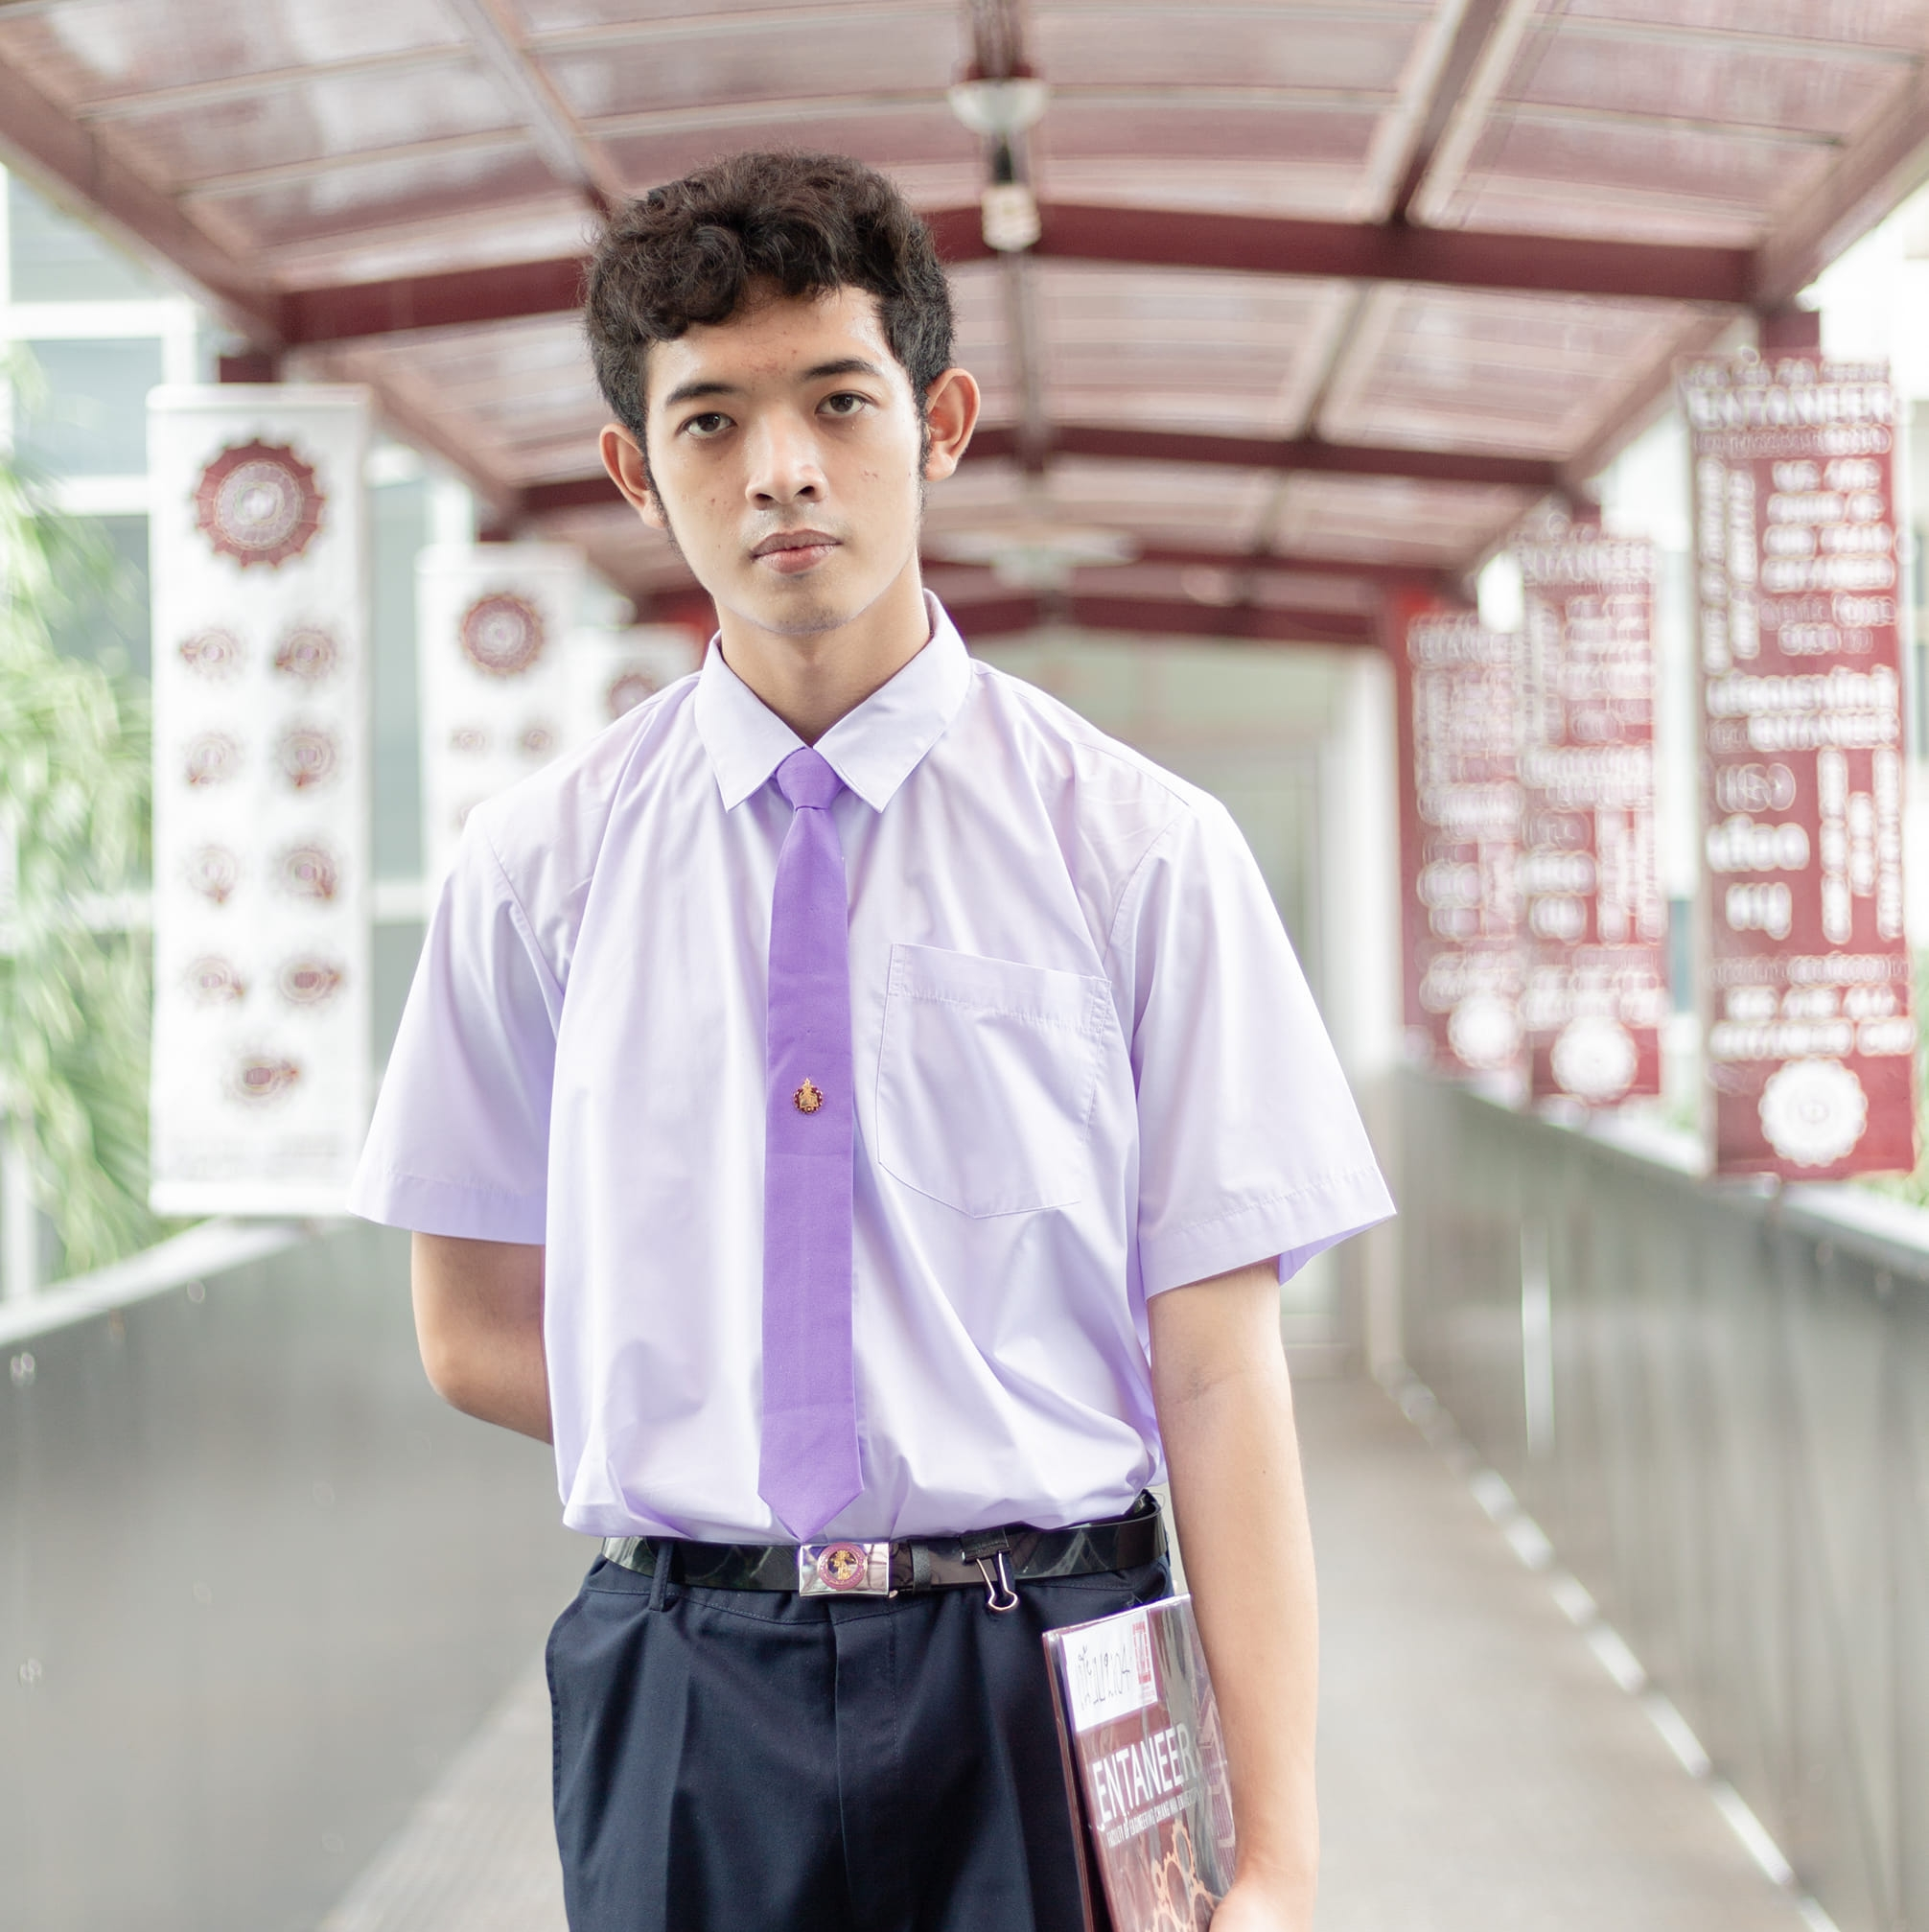
\includegraphics[width=1.5in]{Images/Profile Parinya.jpg}
    \end{center}
    \begin{enumerate}
      \item[] ชื่อ-นามสกุล : ปริญญา ม่วงรอด
      \item[] ระดับการศึกษา : ปริญญาตรี สาขา วิศวกรรมคอมพิวเตอร์ ภาควิชา วิศวกรรมคอมพิวเตอร์ คณะ วิศวกรรมศาสตร์ มหาวิทยาลัยเชียงใหม่
      \item[] E-mail: neabparinya222@gmail.com
    \end{enumerate}

    \begin{center}
      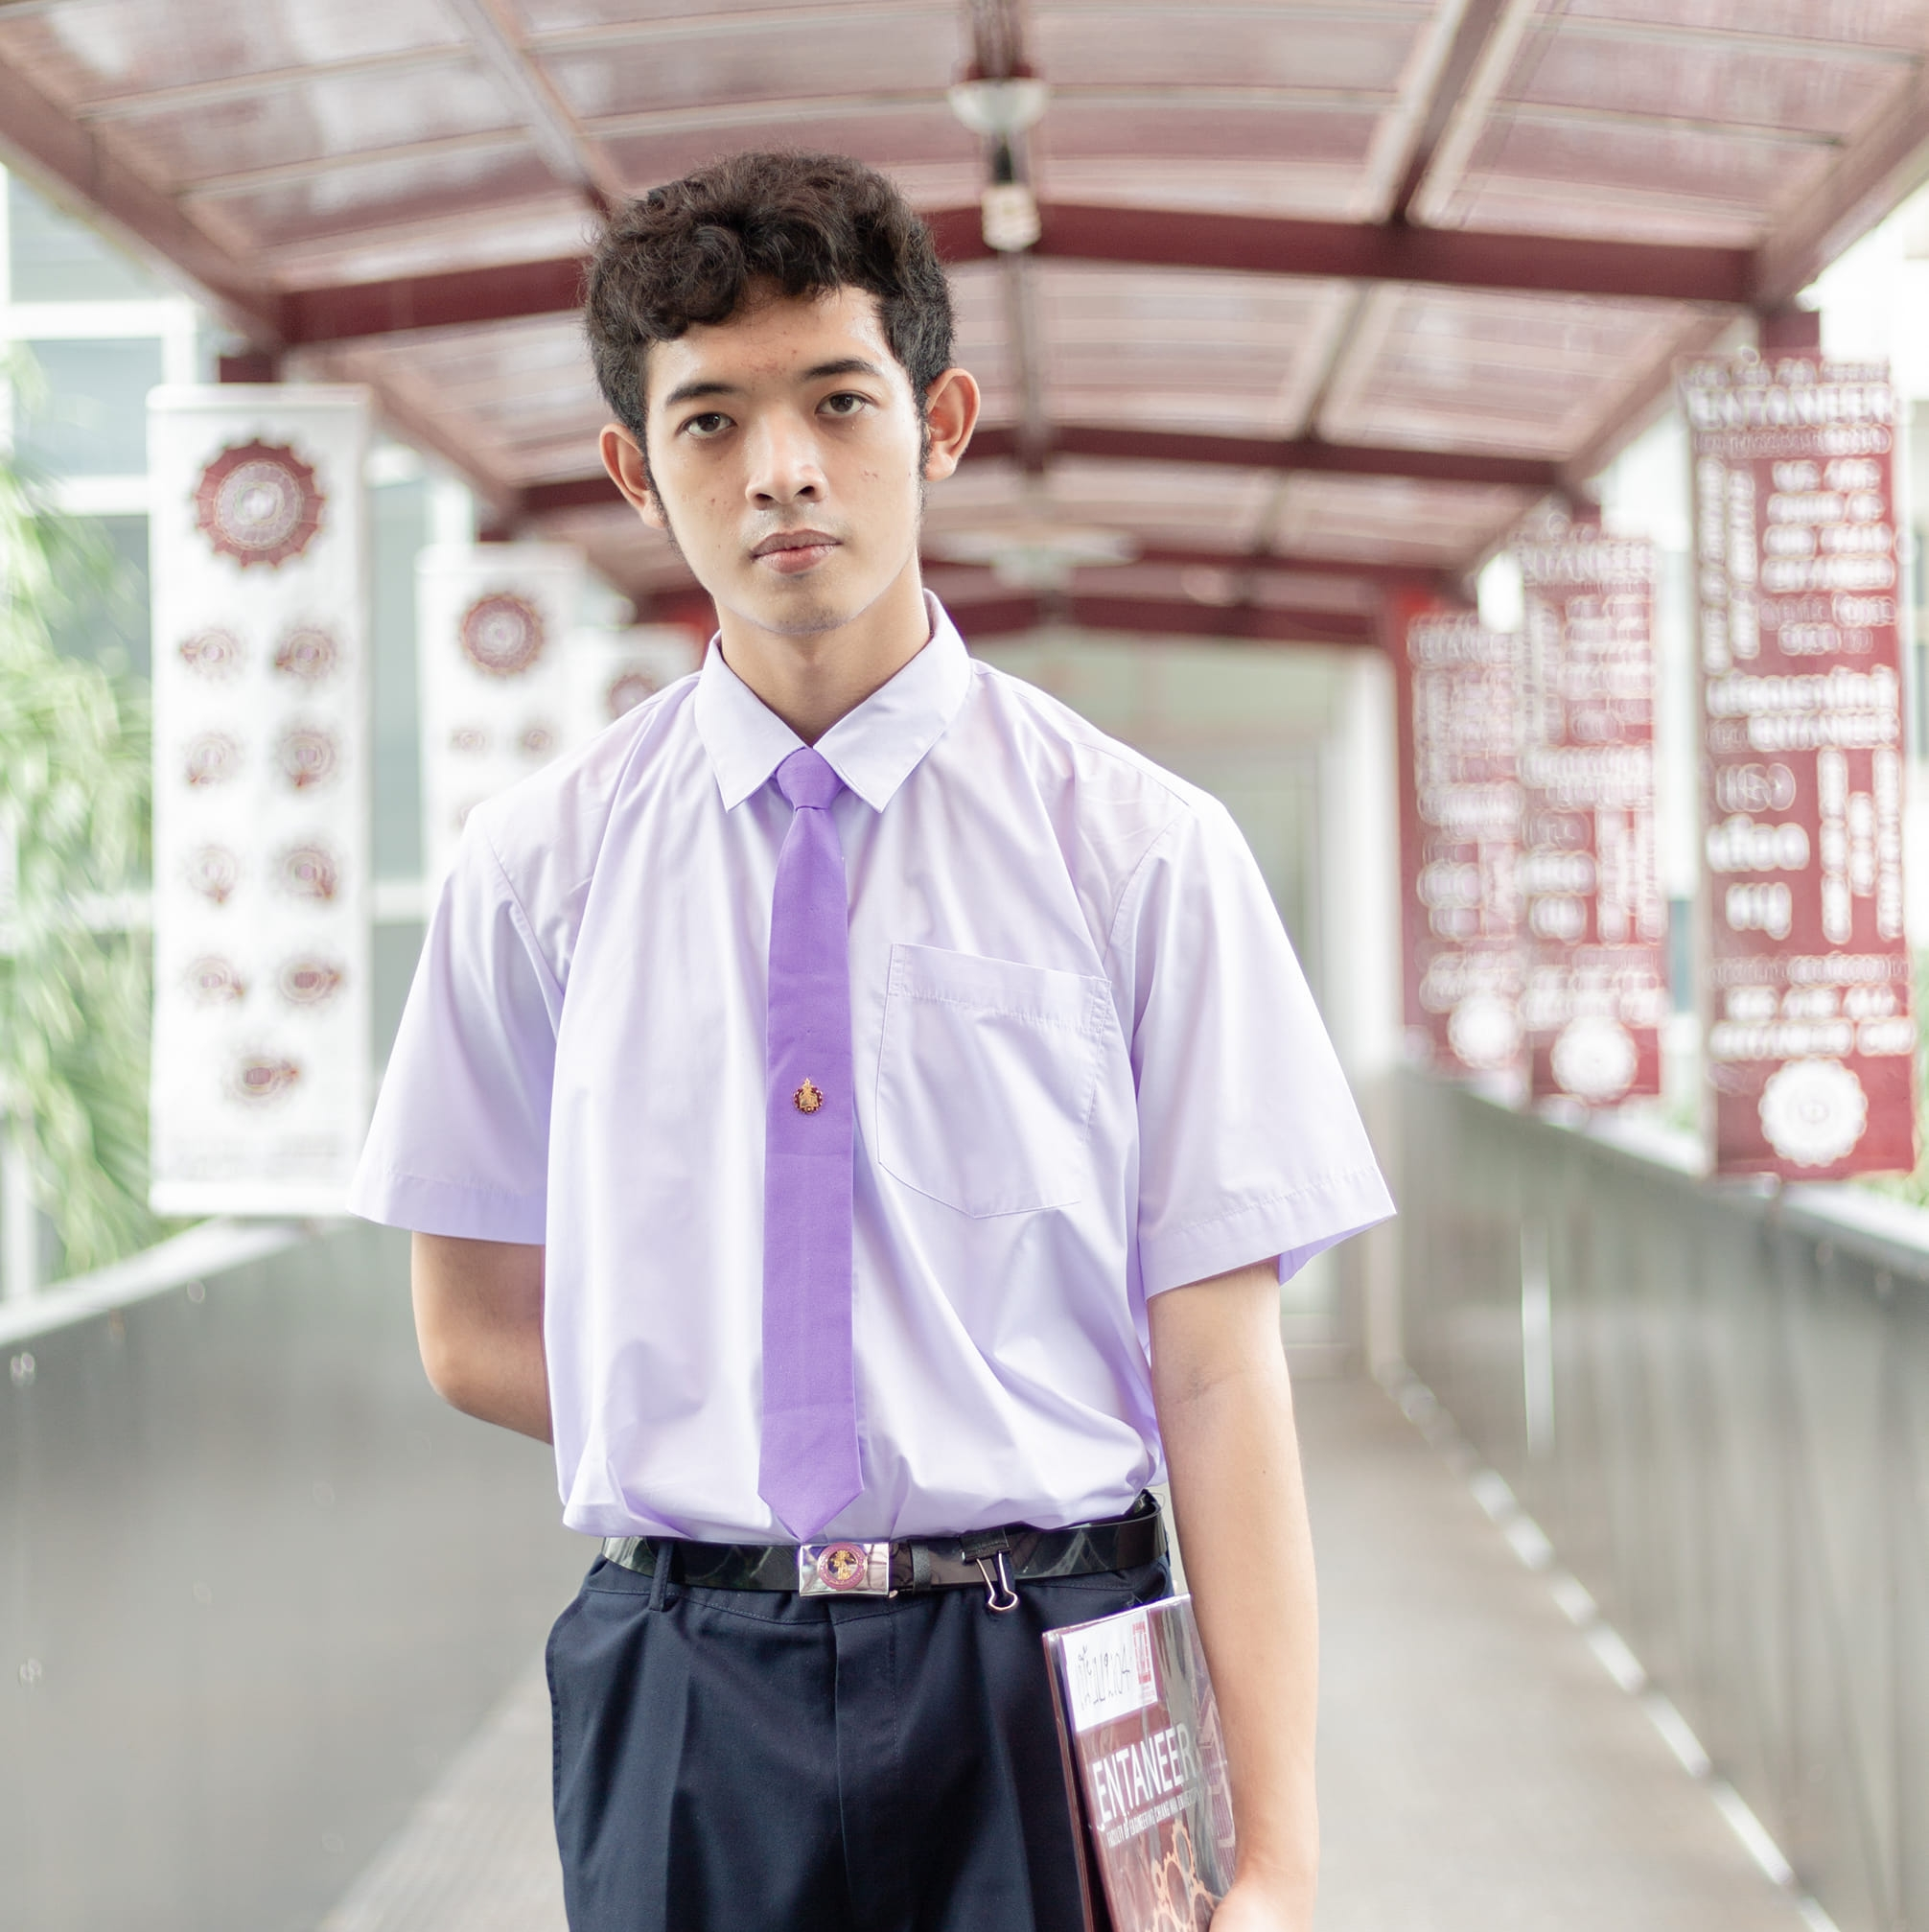
\includegraphics[width=1.5in]{Images/Profile Parinya.jpg}
    \end{center}
    \begin{enumerate}
      \item[] ชื่อ-นามสกุล : วิภาวี วรรธนัจฉริยา
      \item[] ระดับการศึกษา : ปริญญาตรี สาขา วิศวกรรมคอมพิวเตอร์ ภาควิชา วิศวกรรมคอมพิวเตอร์ คณะ วิศวกรรมศาสตร์ มหาวิทยาลัยเชียงใหม่
      \item[] E-mail: wipawee\_watt@cmu.ac.th
    \end{enumerate}
  \end{biosketch}
\fi % \ifproject
\end{document}